\documentclass[12pt]{article}
\usepackage[a4paper, margin=1.25in]{geometry}
\usepackage[hidelinks]{hyperref}
\usepackage[utf8]{inputenc}
\usepackage[nottoc,numbib]{tocbibind}
\usepackage[normalem]{ulem}
\usepackage{fyp-report-style}
\usepackage{graphicx}
\usepackage{subcaption}
\usepackage{float}
\usepackage{pdfpages}
\usepackage{pgfplots}
\usepackage{amsmath}

\usepackage[
    backend=biber,
    style=authoryear,
    urldate=iso8601,
]{biblatex}
\addbibresource{references.bib}

\title{Camera-Projector System as a Hybrid Board Game Model}
\author{Lik Kan Chung}
\idnumber{1780521}
\programme{MSci Computer Science with an Industrial Year}
\supervisor{Professor Andrew Howes}

\wordcount{14,000 words}
% limit 15000
% excludes: title, tableofcontents, figures, tables, abstract, acknowledgements, references, appendices


\begin{document}

%TC:ignore
\maketitle

\tableofcontents
\listoffigures

\setcounter{section}{-1}
\section{Preface}
\subsection{Abstract}
% 200-300 words abstract: problem identified, approach, results, evaluation, conclusion

Board games have long existed in a variety of domains - physical, digital, and hybrid. 
Traditional physical board games allow players to gather together around a board and interact with tangible objects, and digital board games often utilise web apps to display a digital world to players. 
Players of digital board games are restricted to interacting with screens and buttons, while physical games benefit from the tangibility of the physical world. Hybrid board games bridge the gap and offer a compromise to the two otherwise separate domains. Existing hybrid models adapt a physical game by implementing elements of technology, but fundamentally limit the ways a game can be played. 

This project explores a model for implementing hybrid board games as means to allow players to interact with physical the physical domain. A digitally controlled game of tic-tac-toe is brought into the physical domain through the use of a camera-projector system. A camera is used to detect a playing board, and its coloured tokens. Token positions are able to be detected using computer vision techniques and inform a game state, while a projector is used to display this state to a player. 

Prior studies show that there are intrinsic motivations from interacting with physical games. This project has found that implementing physical elements into a digital game shows to intrinsically motivate players to this model. Studies also show games foster social interaction and provide learning experiences. Players found the implementation of technology to enhance the playing experience, and found applications where different people may use it for a variety of reasons, including in education. 

\subsection{Acknowledgements}
Thank you to Professor Andrew Howes for supervision and guidance of this project, as well as to friends for support in testing this model. 

Thanks also extend to members of University of Birmingham Ultimate club, and members of the Computer Science Society for support during this project.

%TC:endignore

\section{Introduction}
% describe general domain, problems, and identified problem, 

% link to references, review intrinsic/extrinsic motivation - build on more in the introduction so it's not so isolated with the rest.. Think about the area of CS the project it concerns - explore the fundamental areas - tangible and HCI. Why does the tangible addition provide an advantage. argue why tangible is more or less motivating. raise this question in the introduction 
% other gians - efficiency - better at picking up games, without worrying about the compression from 3d into 2d. 
% bandwidth - information bandwidth - recruit additional senses - propioception - difference betwen tokens, cast shadows. etc. 
% how important to user perception

Graphical User Interfaces have become ubiquitous in modern computing, making their way into devices since the 1970s and 80s (\cite{ishii2008tangible}).
They form the foundations of modern online board games, allowing players to interact through mouse and keyboard in order to socialise and relax with others. 
However, the point, click, and touch interfaces which many modern devices rely on, is inconsistent with how we interact with ordinary objects in the physical environment around us. 
One such example is the traditional physical board game. 
Tangible games offer haptic interactions, which we lose out on when we cannot take advantage of our dexterity or gain feedback from tactile interactions. 

The physical nature of traditional board games offers players a level of control over how the game is played. 
While it allows players to physically interact with all elements of a game, it also allows groups of players to choose their own tokens or implement their own house rules. 
This may be why many families and social groups prefer to play in a physical domain. 
In a 2020 reflection on ‘Gaming in the Time of COVID-19’, one researcher stated that “The direct contact between players, exchange of artefacts such as currencies, forms, or tokens, is one of the haptic elements that underpins games’ attractiveness.” (\cite{kriz2020gaming})
Physical board games provide comfort, are easy to operate, and are understandable intuitively.
This leads to traditional games being satisfying and appealing for players (\cite{fang2016emotional}). 

Digital board games, on the other hand provide an alternative to physical games by offering elements not available traditionally. 
Online games allow players from across the globe to interact play with each other in real time, and also incorporate an element of customiability to games. 
Players are shown to be more intrinsically motivated to play games, more willing to invest effort, and enjoy games more when they can identify with an in-game character (\cite{birk2016fostering}). 
Studies have also shown that more technologically advanced games have lead to higher player presence and self-reported arousal, while immediate feedback in a game correlates to being more enjoyable (\cite{boyle2012engagement}).

While both physical and digital domains offer advantages when applied to board games, they still have downfalls which could be improved by combining them together. 
Hybrid board games attempt to incorporate the advantages of both, while mitigating the disadvantages which come from the physical or digital spaces (\cite{park2017hybrid}).
Players may be more intrinsically motivated to play a hybrid game for example, where they can benefit from the tangibility of physical pieces, while also being able to customise the graphical elements. 

Existing models lock players into a single game, adapting physical games by adding technological elements. This limits users into the rules of a specific game, which rely on the physical elements which the digital elements are based upon. 
Users do not have the flexibility to create their own house rules as they are freely able to in traditional games.

This project provides a digital-first model for hybrid board games which addresses the issues with existing models. It suggests implementing tangible user interfaces through a camera-projector system, which will enable a digital game software to interface with physical boards and tokens through computer vision techniques. 

This paper reports on the development of the model through background research, where key design elements will be brought forward to produce a specification for an implementation of the model. 
The paper continues to discuss the decisions made in implementation of tic-tac-toe using this model, focusing on the core components of game board and token detection, and game state representation. 
This project proposes an intermediate solution and evaluates the success of this model, suggesting future work and developments. 

% Main body: Literature review, method/approach/specificaton, evaluation/results, discussion

\section{Background}

% - board games are known to be useful in educational settings, but have a wealth of social benefits
% walk through - why people play board games

Board games have found their way into many aspects of modern life. 
In its most basic form, board games, also known as tabletop games, comprise of pieces or tokens placed onto a playing surface\footnote{This surface may be a board, but can also be a table top or desk top where players may gather around} which is typically a board. 
These games often cater to groups ranging in size from 2 to 8, and in some cases larger groups. 
Games can also involve elements of role playing where players must exchange tokens, possessions, or money. 

Despite the requirements for social distance and staying at home caused by the COVID-19 pandemic, reports claim that the global board games market has profited from a combination of people having extra free time as well as economic uncertainty due to events such as Brexit. 
Market research provider Euromonitor International estimated the value of the global market to be worth \$11bn in 2020, with a further \$1bn increase in 2021 (\cite{jarvis2021}).
Their findings suggest that while digital games are a key driver for the games industry, traditional games compliment them, offering an immersive experience for game buyers (\cite{euromonitor2021world}).
With options available for away-from-home entertainment restricted, the demand for at-home entertainment caused a surge of game purchases in early 2020 (\cite{euromonitor2020covid}). However, this has normalised in US markets after stay-at-home restrictions lifted later in the year. 
Nevertheless, trends in digitising traditional games have been predicted to be a strong indicator of success in the future, as games which stay on trend gain more interest from consumers on e-commerce websites (\cite{euromonitor2021uk, euromonitor2021us}). 

\paragraph{Intrinsic Motivation.} % Why people play games as motivation - why people play games.
Intrinsic motivation is when a person is compelled to engage in an activity for the inherent satisfactions gained from it. 
This classic definition suggests that people enjoy fun and challenging activities, regardless of any external pressures or rewards (\cite{ryan2000intrinsic}).
Applied to games, intrinsic motivation stems from the interaction between the player and a game. 
Some studies define intrinsic motivation as an interesting game, while others have defined it as the satisfaction gained from the task. 
These definitions suggest that games which players find enjoyable are likely to gain more play time.

Cognitive Evaluation Theory, a sub-theory of self-determination-theory, provides some factors which suggest why games may be intrinsically motivating to play.
Players may feel satisfaction from the basic psychological need for competence when they experience interpersonal events such as rewards, communication, and feedback.
CET suggests that this only enhances intrinsic motivation where these events are accompanied by a sense of autonomy and actions have been self-determined. 
In order to foster intrinsic motivation for games, they will need to offer a sense of satisfaction from both competence and autonomy. Earlier studies on intrinsic motivation find it is also enhanced where the there is positive performance feedback. 
Choice and the opportunity for self-direction have also been seen to improve intrinsic motivation as players afford a greater sense of self autonomy. 
Activities such as games should also offer novelty, challenge, or aesthetic appeal in order for CET and intrinsic motivation to apply (\cite{ryan2000intrinsic}).

Where activities do not offer these elements, intrinsic motivation does not apply. 
Events such as tangible rewards, threats, deadlines, directives, and competition have also been seen to diminish intrinsic motivation. 
Extrinsic motivation may address these issues, where activity engagement is performed in order to attain a separable outcome. 

\paragraph{Educational Benefits.} Aside from playing games as a social device, board games have also shown to be useful in educational settings. 
In young children and especially those from low-income backgrounds, games which are numerical in nature have shown to improve numeracy skills. 
Games which are mathematical and linear in nature have improved key aspects of early numerical understanding. 
These numerical games have benefits in concepts such as knowledge of numerical magnitudes, counting, numerical identification, and arithmetic
Snakes and ladders has been commonly cited as a game which is simple and easy to learn, while improving these skills in children (\cite{siegler2009playing}).

Benefits have also been demonstrated in games for adult learners. 
Adult education is underpinned by the fact that there is always something new to learn, and that there are always opportunities to learn with and from others. 
Studies show that game-based learning provide different interdisciplinary experiences which allow learners to learn in different ways. Games afford learning experiences that allow mistakes without real-life consequences; provide chances to discover personal relevance; and can be used at an individual's own learning pace (\cite{boghian2019game}).

\begin{figure}[h]
    %TC:ignore
    \centering
    \includegraphics[width=0.5\textwidth]{images/figures/fig1}
    \caption[CATAN]{CATAN: An example of a  Eurogame in which players compete for resources to build and develop holdings. The game is played on hexagonal tiles with cards and wooden pieces representing resources and buildings.}
    \label{fig:catan}
    %TC:endignore
\end{figure}

\subsection{Board Game Domains}
The traditional board game has existed various formats and styles for many centuries. 
Games started to grow in popularity during the 1990s and 2000s, and the term 'Golden Age' has since been used to refer to its success (\cite{guardian2014,konieczny2019golden}). 
Physically printed games have become more readily accessible with the growth of online retailers providing wide ranges of games and fast delivery times. 
The internet and social media has helped in games' marketing, and digital versions of physical games have also been said to provide a taste of a game, with many players going on to buy the physical version afterwards (\cite{guardian2014}).
Meanwhile, the rise in popularity of board game cafes has reinforced the physical board as a gaming media, while also providing a social space for players to meet (\cite{konieczny2019golden}).

Modern board games are often categorised into two styles: European and American.
Eurogames\footnote{European-style board games, also known as German-style games.} are generally strategy based, revolving around interaction with physical components and resources.
Examples such as CATAN\footnote{Formerly \textit{The Settlers of Catan} (1996) and \textit{Die Seidler von Catan} (1995), Klaus Teuber} (Figure \ref{fig:catan}) paved the way for Eurogames and have developed expansions and digital versions. 
This style of game often involves indirect conflict such as competition through limited resource pools, as opposed to American style games which typically engage through aggression and luck to entice drama and a story.
However, in the last decade, the lines between the styles have blurred and many games implement concepts which cover both styles (\cite{guardian2014}).
Board games, therefore have many elements which make up the setup and play-through of a particular game. These elements impact on how players will experience a game and how much they enjoy it overall.

\subsubsection{Elements of a Board Game: The Role of Chores in Social Play}
Social interactions are key to the experience of board games, and often are fundamental to the gameplay. 
Games have similar elements before, during, and after gameplay, which dictate the actions which players must make, and therefore influence the social interaction that exists between players by dictating common topics of conversations and debates, as well as providing a source of jokes and points of reference for gestures such as pointing. 

\textcite{xu2011chores} undertake an empirical study and analyse a series of gaming sessions between a group of players, identifying five categories of gameplay mechanics which influence four types of social interactions. 
The study focuses on social play from co-located player social play experiences which involves both physical and digital media. 
Sessions are analysed with Interaction Ritual theory as a basis for the co-located face-to-face interaction which many board games rely on. 
IR theory identifies four key factors for successful social interactions:
\begin{itemize}
    \item \textbf{Bodily co-presence} - Players grouping together in the same space
    \item \textbf{Barrier to outsiders} - A sense of who is partaking and who is not
    \item \textbf{Mutual focus of attention} - Awareness of other player's attention focus on a common object or concept
    \item \textbf{Synchronisation} - A shared mood or emotion within the group
\end{itemize}
Bodily co-presence and barriers to outsiders concern the concept of the gaming session itself.
It enforces that the games are played within a social setting, where the location and membership of the players within the group are a basis on how game elements and mechanics are interacted with. 
The latter two factors deals with the social interactions within the game setting, in which players focus on game elements and mechanics, while the players collectively convey emotions based on events within or caused by the game.
These factors were observed in the game elements which Xu et al. found: 
\begin{itemize}
    \item \textbf{Chores} - Tasks which are required to enable gameplay and maintain correct game states
    \item \textbf{Reflection on gameplay} - reactions or reflections about a move or sequence of gameplay events
    \item \textbf{Strategies} - discussions before a move or play 
    \item \textbf{Out-of-game} - discussions on topics outside of the game 
    \item \textbf{Game itself} - discussions about the game itself
\end{itemize}

Chores are fundamental to all games as they facilitate the tasks which are required to play though a game.
Tasks such as setting up a board; shuffling and distributing cards, tokens, and resources; moving tokens; rule enforcement; and bookkeeping are elements which establish a structure and common understanding of a game. 

These tasks are often simple to complete without much thought, and are prime targets for automation in digital games. 
However, Xu et al. find that chores facilitate rich social interactions which may not exist if they are automated. 
While chores can be simple, they can be often time consuming. 
This slow down in gameplay afforded alternate interactions to arise, where the change in pace creates time which players filled with other activities. 
Xu et al. find evidence to show that cooperation with chores enhanced players' physical co-presence as well as their awareness of other's actions. 
They found several instances where chores contribute to successful social interactions. 

Board games usually include physical objects to guide a journey through a game, whether they are tokens, dice, or cards. 
Interacting with these objects usually means physically handling them and performing an action which other players are able to observe.
It is these actions which attract attention of other players, who may comment or react to these gestures. 
Bodily co-presence creates these opportunities for players to observe and react to events. 
Physical objects therefore allow players to influence conversation, for example where a dice roll may incite reactions from players who did not physically interact with the dice. 
Even when there is no significant event happening, co-located players track each other's motions and how they act, and also make themselves trackable to other players. 

In turn based games, a player may have to wait some time between their turns. 
This time, again, fosters conversation which reflect on their gameplay, out-of-game subjects, or the game itself. 
These conversations change as turns are played in turn based games. 
Players may join a centrally focused conversation and switch to a threaded side discussion, which prevents players from dominating a conversation. 
This is primarily caused by the centre of the group's attention rotating around players as they play turns. 

Physical games often provide the advantage of allowing players to flexibly enforce rules. 
"House Rules" are rarely seen in digital games, as rules are often computed precisely with no deviation since rule enforcement is often error prone when handled by humans. 
Opportunities to create social interactions, where all players are involved, arise in situations where there may be disagreements or hesitations on rules. 
Social negotiation in this instance advantages from altering a game's rules to provide a basis for a more enjoyable social experience.

Similarly, these situations afford opportunities for collaborative learning. Interactions among players support the learning experience of a particular game, and allows players to create their own interpretations and feelings about a particular element in a game. It is clear that flexibility in game rules is required in order to foster social negotiation and agreement, but they must still be rigid enough to allow opportunities for players to collaboratively learn game mechanics. 

Xu et al. discuss the impact of chores on social interactions to a significant extent, and argues that chores as an element of board games facilitates other elements through social interaction. 
These interactions are ones which are easily automated by a digital game, so it is therefore important to carefully balance elements of a game which should be automated, and which should be left for players to interact with physically. 
It is these physical interactions which create a common grounding for players to understand a game state and the social dynamic within the group. 
This common grounding can therefore trigger other social interactions, and make chores enjoyable and fun. 

% - comparing physical and digital games
\subsubsection{Physical versus Digital Games}
\textcite{xu2011chores} focus on the social interaction based around traditional physical board games. 
However, modern technology finds its way into the gaming experience when digital devices are so widely used in everyday life, making it one of the most popular leisure activities globally. 
Inevitably, digital games become ubiquitous in many adolescents' lives (\cite{fang2016emotional}), as well as becoming a past-time for many adults (\cite{boyle2012engagement}). 
While physical games foster social interaction in a co-located space, physical environments often differ greatly when players turn to digital games. 
The differing use of technology thus changes the social experience, and may accommodate different emotional reactions. 

\textcite{boyle2012engagement} review fifty-five papers on engagement in digital games. 
They find that digital games alone can have a significant impact on a player's emotions. 
One advantage of digital games is that human players are able to play with computer controlled players where traditional board games offer no comparable mechanism. 
Boyle et al. find studies which state that players playing with other humans feel stronger presence\footnote{A player's perception of being mediated within the environment of a game} and enjoy a game more.  
This may be explained by advancements in technology which allow for better interactivity, animations, or download speed.
These developments have also independently been shown to lead to similar effects of presence and enjoyment. 
Player presence was found to be the most important predictor for game enjoyment within players, although it is not a good indicator for overall play time.

The flexibility of digital games has also shown to impact emotions. 
Games which have suspenseful elements are more enjoyable than those without, while the use of sound and music could also impact a player's feeling of immersion, tension, or competence.
Immediate feedback is another feature afforded by digital games. 
Studies show that when immediate feedback, such as feedback about actions made in game, was reduced it caused player effectance to reduce and thus reduced enjoyment overall. 

Finally, Boyle et al. reviewed motivations for playing digital games. 
The need for companionship and preferring to play digital games over being with friends was attributed as a need which playing games meets for adolescents, as well as being fun and challenging, and being a stress relief. 
This differs from the social interaction seen when playing physical games, where co-location was a key factor in the types of interaction exhibited. 
In digital games, players freely develop relationships within games in a virtual world, rather than using a game as a physical focus of attention on which social interactions happen around.

\begin{figure}[h]
    %TC:ignore
    \centering
    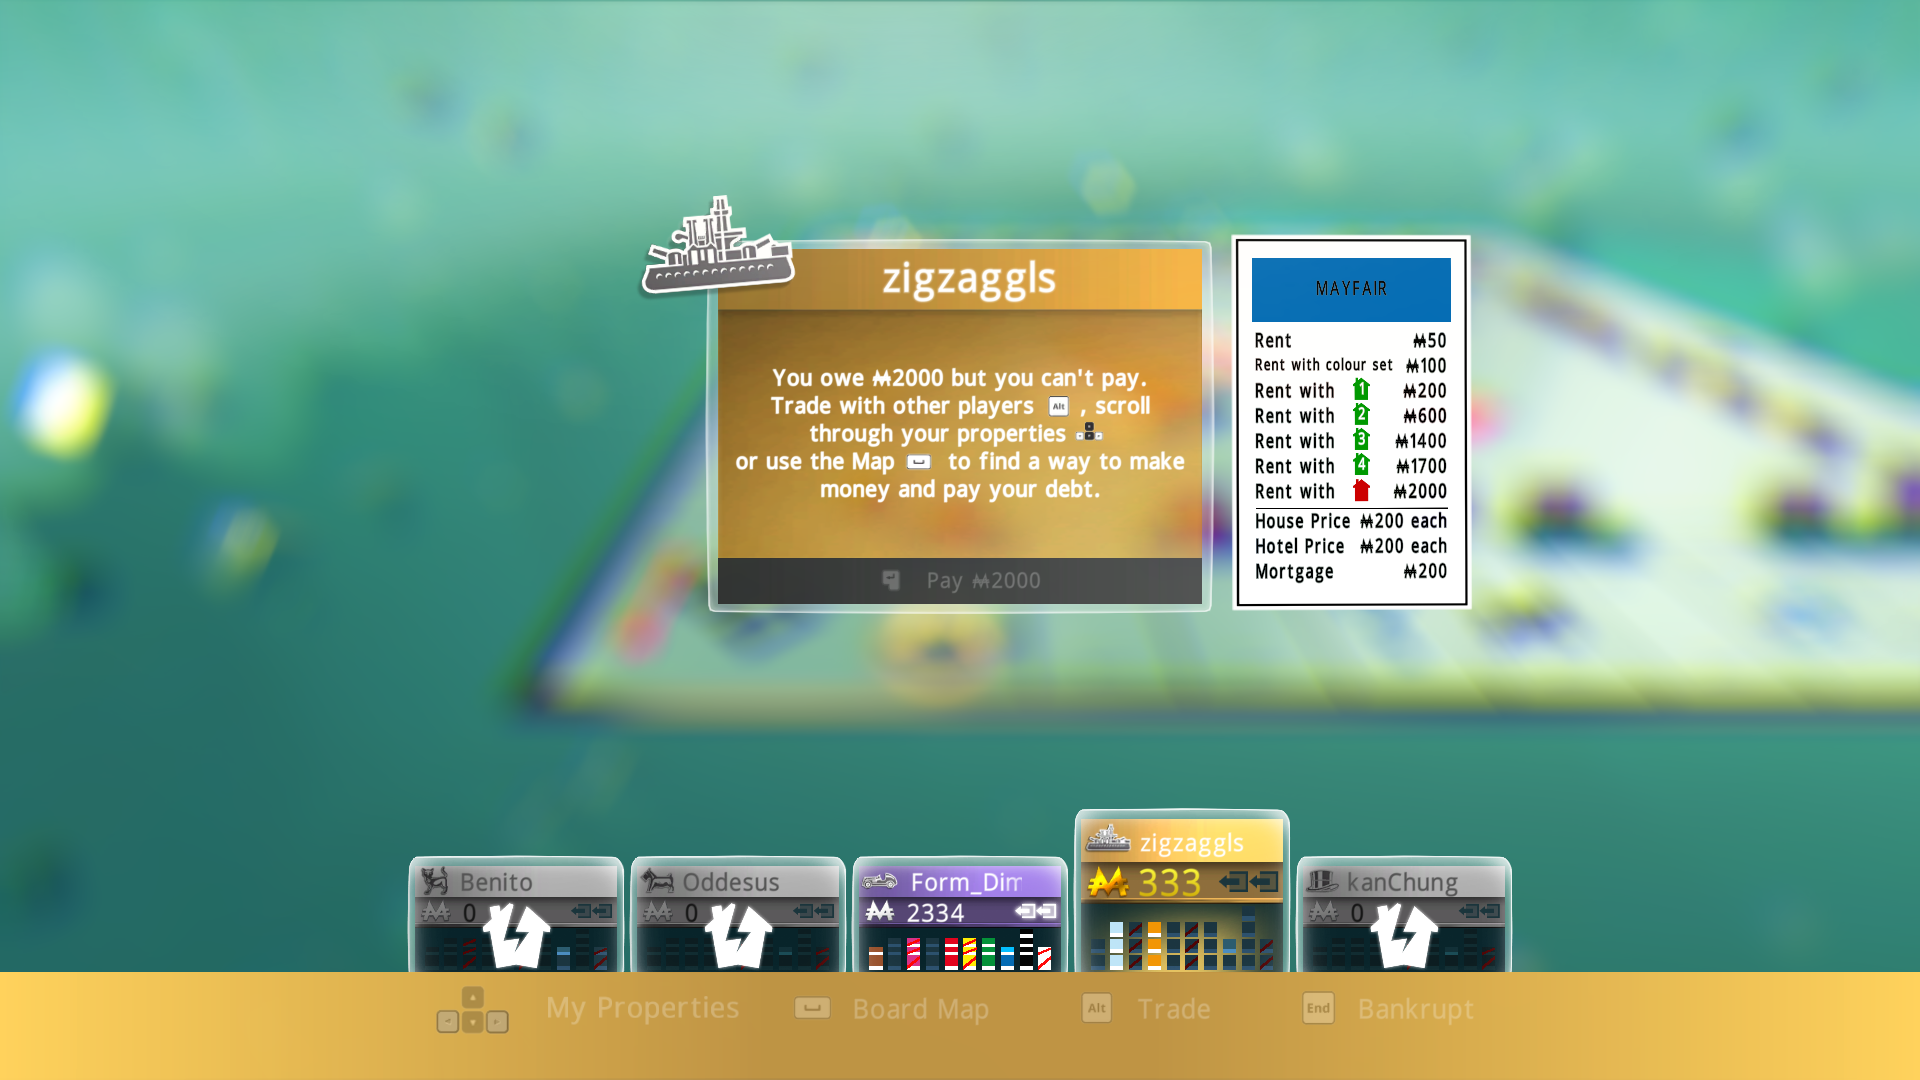
\includegraphics[width=0.8\textwidth]{images/figures/fig2}
    \caption[A screenshot from Monopoly Plus]{A screenshot from Monopoly Plus: The game indicates to a player that an action must be completed before the game can continue. The popup instructs the player: "\textit{You owe \dout{M}2000 but you can't pay. Trade with other players, scroll through your properties or use the Map to find a way to make money and pay your debt.}"}
    \label{fig:monopolyplus}
    %TC:endignore
\end{figure}

\paragraph{Adaptation from Physical into Digital Games.} Digital board games, however, offer different styles of interactions than the majority of digital games. 
Many games have been adapted from successful physical versions into a digital world. 
Monopoly is a classic example where chores in the traditional version have become semi or fully automated in a digital version. 
Monopoly Plus (\cite{monopolyplus2017}) differs from the traditional version of Monopoly (\cite{monopoly}) by dictating the play-through of the game. 
Players in the digital version must start a dice roll with a button press, and its value is calculated by the computer. 
The digital version also enforces rules (Figure \ref{fig:monopolyplus}), including ones which occur less frequently.
This limits players' exposure to opportunities which invite social negotiation, or collaborative learning through creating house rules or clarifying existing rules.

When comparing the traditional and digital versions of games, namely popular physical games Monopoly and Jenga, \textcite{fang2016emotional} found the physical games to be equally or more superior in all aspects, with a tablet version of the game scoring lower than the desktop digital version. 
The physical game triggered the highest visceral preferences of attraction in attributes relating the to the form, texture, colour, and impression of the game. 
This tangible nature of the physical interface therefore scored highest in satisfaction survey questions. 
The physical game also scored well in factors relating to comfort, ease of operation, and ease of understanding, showing that the simple nature of physical games are easier to play without learning how to interface with them. Technology therefore has an opportunity to innovate with new tupes of interaction and intuitive operations. 
Fang et al. reccommend that digital games should take advantage of advances in technology, as while they cannot replace physical and social interactions around traditional games, they are in a prime position to innovate for new games and provide new leisure experiences. 

% - motivation in digital games
\subsubsection{Motivation in Digital Games}
While traditional games are preferred for well established games in the market, elements of digital games can be attractive for games which are able to innovate. 
Digital games allow flexibility to represent artefacts from the game in ways which can change over time, unlike traditional games where the objects used to play games are the same as when they are manufactured. 
Environments, player avatars, and inventory items are all objects which require design in both physical and digital games.
This creates the scope for these elements to be customisable by both players and developers, allowing a subset of players to see different designs. 

Birk et al. investigate whether allowing players to identify with avatars in digital games fosters intrinsic motivation (\cite{birk2016fostering}).
Outside of games, character identification\footnote{The degree in which a person empathises with a character.} has shown to increase enjoyment in media.
Unlike film or television, games introduce an aspect of autonomy and agency where a player is able to make decisions which directly affect a player or object. 
Players are able to have a sense of presence in dynamically evolving outcomes for an avatar which is not rigidly set to a defined storyline. 
Balancing the storyline and the degree of agency a player is able to experience is essential to creating an enjoyable game. 

Birk et al.'s work finds that in a infinite runner game, players who customised an avatar showed more signs of identification with the game. 
They also showed that this increased identification increased in-game needs and intrinsic motivation. 
This intrinsic motivation has benefits for the play experience, but there are also possible economic benefits. 
It is suggested that players who are more intrinsically motivated to play a game would be more likely to spend time playing the game and recommend it to others, growing a game's player base. 
Therefore, this work indicates that a game which allows players to customise graphics to their preference may invoke intrinsic motivation. 

\subsection{Related Work}
While graphical user interfaces are ubiquitous in modern computing, they are restricted in what they can offer. 
GUIs represent data through pixels, imposing a limit in resolution and detail.
\textcite{ishii2008tangible} finds these devices to be inconsistent with the world we live in, and how we interact with objects every day. 

\subsubsection{Tangible User Interfaces}
Tangible user interfaces bridge the gap between a 2D display on a screen, and ordinary objects. 
They offer the advantage of haptic interactions, which is a significantly different form of interaction from GUIs (\cite{ishii2008tangible}). 
It is the aim of TUIs to fit seamlessly into a user's physical environment and make available natural gestures and interactions. 
A tight coupling of object manipulation and digital representation is beneficial to creating a usable experience for users. 

TUIs interject digital information into the physical domain through tangible and intangible representations. 
Users are able to input into the system though physical objects, which represent the system in a tangible way.
These inputs are interpreted by computer systems which store an internal representation, and may provide some outputs. 
TUIs are limited in that they usually are not capable of extensive tangible outputs. 
While GUIs are able to change pixels on a screen, TUI interfaces are generally incapable of manipulating physical objects. 
However, this may no longer be the case as developments in robotics and 3D printing have come a long way since Ishii described these intangible representations. 

Physical objects are somewhat unconstrained in what a human user is able to do with it.
A usable TUI must constrain objects into what is reasonable. 
In order for a system to be easy to use and learn, a design must base interactions on what is already well understood about an object. 
In the example of board games, it is culturally common that dice can be rolled to generate a random number, and tokens can be picked up and moved to mark a player's location on a board. 
These common gestures disambiguate how users should interact with a TUI. 

Therefore choosing what elements of a system should be represented physically, and which should be digital is important in creating tangible interfaces. 
Tangible hybrid board games can take advantage of both physical and digital domains, but must remain usable if the game is to be enjoyable. 
Mundane tasks such as board setup should be automated and implemented digitally, while objects which are fundamental to making strategic choices should be physical (\cite{ip2011virtualize}).

\subsubsection{Hybrid Board Games}
Hybrid board games have been available in many forms along side their traditional counterparts. 
However, many current implementations adapt a physical game into one that incorporates digital elements. 
While traditional games have already shown to be preferred over digital and tablet versions, there are few implementations which offer digital games a venture into the physical domain. 

Hybrid Monopoly is one such investigation which adapts a physical game with electronics. 
\textcite{park2017hybrid} reworks a traditional game board to incorporate hardware which is able to sense the presence of objects such as tokens or cards. 
Their model is built around a tablet which controls the game, and offers an API which allows a designer to change and adapt the game.

Their work allows users to implement house rules while playing, but it is restrained by its implemented technology. The types of games which could be implemented is restricted by the layout of the hardware and its reliance on a central tablet. 

\subsection{Conclusion}
Games are fun and allow players opportunities engage with each other socially. 
They can offer some benefits in educational settings, while players are also attracted to play games intrinsically. 
Games therefore have an important role to play in building relationships between players by allowing discussions to form around or as a result of events which may happen while playing.
These interactions should be preserved as they form a basis of what makes games enjoyable.

Current work in tangible user interfaces are able to detect objects in various ways, while existing hybrid board games adapt a physical game with electronics. While informed by this work, this project finds that there is scope to implement a hybrid board game model which uses an overhead camera-projector system to provide players with an instance of a board game. Players will be able to interact with a system which presents a game to the user, and the player will be able to make moves to play a game.

\section{Design}
With consideration of previous work, including research on enjoyability of games, and design of hybrid board games, requirements are derived for for a camera-projector hybrid board game implementation, with assumptions and limitations in mind.

\subsection{Assumptions}
As this is fundamentally a project based around peripheral devices and physical objects, there are some assumptions which are made about the physical world. These assumptions inform the design requirements, and may also create some limitations.

\paragraph{A game board is white and is played on a flat surface.} A board game is played on a board, so it is assumed a board will be placed on a surface which is flat and easily accessible for players. It is also assumed that the board is square in shape and is white in colour.

\paragraph{Tokens are a specific colour and do not change in shape or size.} Tokens are physical objects which players can manipulate, but it is assumed that they will be constant and cannot change in colour, shape, or size. 

\paragraph{The camera and projector can be positioned in any orientation.} The camera and projector are hardware devices that are commonly built to be mounted such that they are pointed horizontally towards an object, i.e. a person or screen. 
It is assumed that the mounting hardware of an implementation will not limit how the peripheral devices are positioned. 
Similarly, it is assumed that these peripherals are connected as devices on a computer which can run software.

\paragraph{Players are physically able to interact with physical objects.} A feature of tangible-user interfaces is that it can both limit and help users with disabilities who may otherwise have issues using graphical user interfaces. 
This project assumes that users are able to pick up and manipulate physical objects on a table surface. 

\subsection{Requirements}
Taking the listed assumptions into mind, an implementation of the goals of this project considers the following requirements. These goals are:
\begin{itemize}
    \item To implement a system which utilises a camera and projector, and
    \item Use this system to provide a hybrid board game experience with a user
\end{itemize}

\subsubsection{Functional Requirements}
\begin{enumerate}
    \item A simple game is implemented which uses a game board and tokens
    \item A camera is able capture an image of a game board and tokens on the board
    \item Coordinates of a game board and tokens are able to be calculated
    \item Game board and token coordinates can be mapped to coordinates of a game
    \item Positions of tokens can be used to determine a move or game state
    \item A game state is stored internally
    \item A visual representation of the game state is displayed
    \item A projector displays the visual representation of the game state onto a board
    \item Multiple game tokens can be detected on a game board
    \item Game tokens of different colours can be distinguished between
    \item Only the most essential game chores are automated
\end{enumerate}

\subsubsection{Non-Functional Requirements}
\begin{enumerate}
    \item Images from the camera should have be processed in near real time, i.e. the camera-detection process should not lag
    \item Game pieces, such as tokens, are simple objects that can be easily sourced
    \item Game piece moves cause visual feedback near instantaneously
    \item Control of the game state is easy to learn, i.e. gestures such as moving a token is intuitive
    \item Setup and configuration should be straightforward
    \item Additional games can be implemented easily with the same peripherals and physical objects
\end{enumerate}

\subsection{Methodology}
These requirements detail what this project will implement. 
The system is designed as a loop from the player making a move, which is interpreted and processed by the software. 
The processing causes updates to an internally stored game state, which is then displayed by the projector. 
In theory, any game can be implemented, but tic-tac-toe is chosen due to its simplicity. 

\begin{figure}[h]
    %TC:ignore
    \centering
    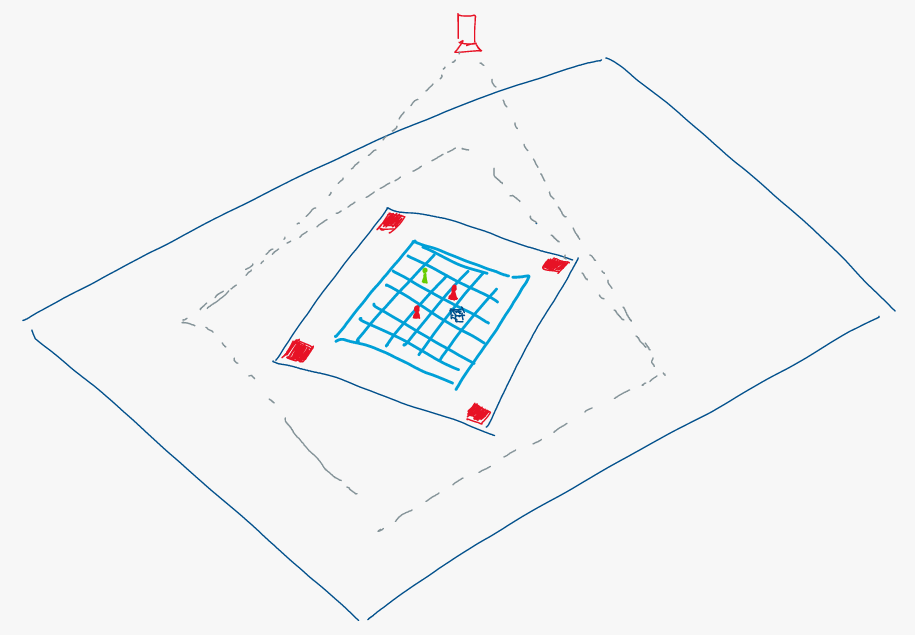
\includegraphics[width=0.8\textwidth]{images/figures/fig3}
    \caption{Initial design sketch}
    \label{fig:designsketch}
    %TC:endignore
\end{figure}

\subsubsection{Physical Game Representation}
From research in current work, games such as Hybrid Monopoly (\cite{park2017hybrid}) in academia and Monopoly Super Electronic Banking (\cite{monopolyelectronic}) available commercially limit the player to a single game. 
This means that players who invest in a product are limited to that game. This project attempts to solve that problem by using a blank white board, and projecting the game's visual design onto it. 
Figure \ref{fig:designsketch} shows an initial design sketch where a board is placed on a table with the camera-projector system mounted directly above, with the direction of gaze facing downwards.

The visual design in of tic-tac-toe is a 3x3 grid, which will be displayed on the main screen of the computer.
The projector mirrors the computer's display onto the board, so will project the grid. 
For this two player game, each player can use a coloured token to make their moves. 
A player's occupation of a space is traditionally denoted by a 'O' or 'X'. In this system the game will colour the square to show the player has selected that square. 
Players move pieces by physically picking them up and moving it to their next desired location. 
The rules will not be displayed to the user and the instructions detailing a next move are not calculated. 
This also allows players flexibility to create their own house rules, adding additional players for example.
This means that only the logic to interpret a move, and calculate a game state are required. 

Using simple tokens to represent a player is a straightforward concept to comprehend since it is a common object found within board games. 
This makes the game easy to pick up and start playing, with a shallow learning-curve. 

\begin{figure}[H]
    %TC:ignore
    \centering
    \begin{subfigure}{0.65\textwidth}
        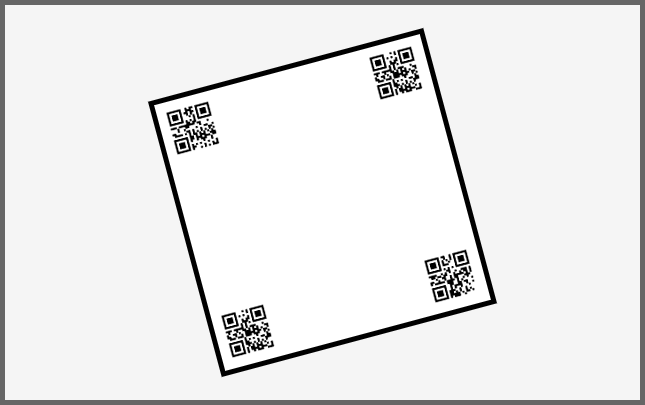
\includegraphics[width=1\textwidth]{images/figures/fig4a}
        \caption{Image capture of game board on a playing surface}
        \label{fig:boarddetectiona}
    \end{subfigure}
    \begin{subfigure}{0.65\textwidth}
        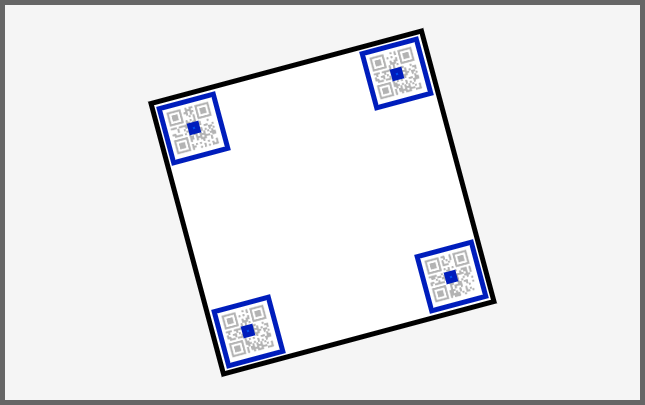
\includegraphics[width=1\textwidth]{images/figures/fig4b}
        \caption{Image capture of board with detected QR codes labelled}
        \label{fig:boarddetectionb}
    \end{subfigure}
    \begin{subfigure}{0.65\textwidth}
        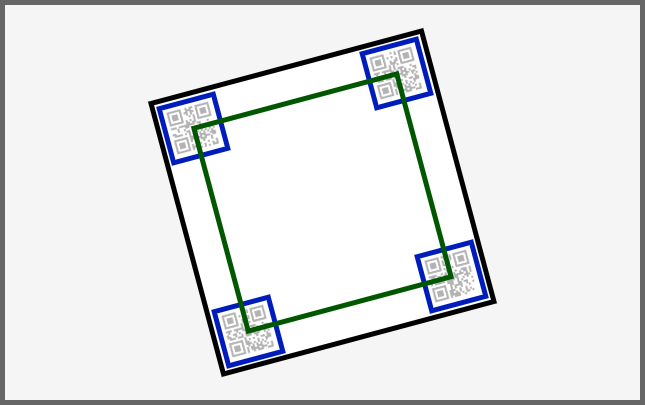
\includegraphics[width=1\textwidth]{images/figures/fig4c}
        \caption{Image capture with a rectangle drawn with QR codes as vertices}
        \label{fig:boarddetectionc}
    \end{subfigure}
    \caption{Process of game board bounds detection}
    \label{fig:boarddetection}
    %TC:endignore
\end{figure}

\subsubsection{Board and Token Detection}
In order to correctly calculate the position of a piece the objects the camera captures an image which is processed. 
As shown in Figure \ref{fig:designsketch}, the playing surface is a board with QR codes (red squares) printed in the corners. 
These codes are static and do not change, so they will be used to determine the position of objects on the playing surface.

An image of the playing area, which includes the board with the QR codes, is scanned to find the coordinates of the codes within the camera coordinate frame. 
The four codes which are detected can then be used to find a playable area in the image. Figure \ref{fig:boarddetection} shows the process:

\begin{enumerate}
    \item An image is captured of the playing surface which includes the board and its QR codes (Figure \ref{fig:boarddetectiona}).
    \item The image is scanned to find QR codes and their coordinates in the image. The blue rectangles in Figure \ref{fig:boarddetectionb} denote QR codes\footnote{In Figure \ref{fig:boarddetectionb} and Figure \ref{fig:boarddetectionc}, the QR codes are a different colour to Figure \ref{fig:boarddetectiona}. This is only done to highlight the drawn rectangles in blue and green.} which have been found in the image.
    \item The centre of each rectangle is found by averaging the minimum and maximum $x$ and $y$ coordinates. The centre point is also shown in Figure \ref{fig:boarddetectionb}.
    \item The four centre points define points near the edge of the board. This creates a rectangle which is shown in \ref{fig:boarddetectionc} where the vertices are the four QR code centres. 
\end{enumerate}

\begin{figure}[H]
    %TC:ignore
    \centering
    \begin{subfigure}{0.4\textwidth}
        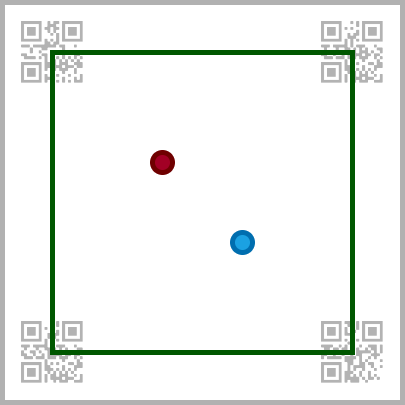
\includegraphics[width=1\textwidth]{images/figures/fig5a}
        \caption{Two tokens placed on the board within the area to search}
        \label{fig:tokendetectiona}
    \end{subfigure}
    \begin{subfigure}{0.4\textwidth}
        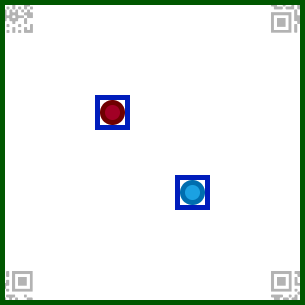
\includegraphics[width=1\textwidth]{images/figures/fig5b}
        \caption{Rectangles drawn bounding the two tokens detected on the board}
        \label{fig:tokendetectionb}
    \end{subfigure}
    \caption{Process of game token detection}
    \label{fig:tokendetection}
    %TC:endignore
\end{figure}

Since four points at the corners of the board are found, a playable area within the rectangle is found. 
It is therefore possible to detect game token pieces within this section of the image. This process is detailed in Figure \ref{fig:tokendetection}:

\begin{enumerate}
    \item The previously captured image from board detection is cropped to the searchable area (Figure \ref{fig:tokendetectiona}).
    \item The cropped image is searched for the shape of the token. A blue rectangle shows the bounding box of the found pieces in Figure \ref{fig:tokendetectionb}.
    \item The colour of the piece can be calculated by again cropping the image to the bounding box and computing the colours of the pixels by average RGB\footnote{Red, green, and blue colour channels} values.
\end{enumerate}

\subsubsection{Internal Game Representation}
Since the coordinates of the board and tokens can be found, the tokens' position on the board can be calculated. 
With a relative position, a tic-tac-toe move can therefore be derived. 
As tic-tac-toe is a simple game, a simple data structure can store the game-state. 
A 2D array is sufficient to store the colours of each grid location. 
Once the data structure is updated from token and colour detection, the display output can be updated which is projected onto the board. 
If there is a winning state, then that is displayed with a message to the players. 
Players can then clear the board and play again. 

Previous findings suggest that chores can be automated, but the extent of automation should be limited in such a way that it does not detract from the playing experience.
This design automates a significant proportion of the chores for the player. 
However, tic-tac-toe is a game with few chores, so the chores automated for the player are:
\begin{itemize}
    \item Drawing the grid lines
    \item Marking the move played in each tile of the grid
    \item Determining if there is a winner
\end{itemize}
This leaves freedom for the user to create their own ways to play. 
For example, there is no restriction that players must take alternating turns. 

Players receive instantaneous visual feedback that their move has been played, so then another move can take place. 
The players would be able to perceive that the physical and internal representations of the game are tightly coupled, meaning there is confirmation a move is complete and there is no slow down in play time.

\subsection{Limitations}
\paragraph{Games vary in complexity.} Since this project is evaluating the projector-camera system as a model to implement hybrid board games, the actual game implemented is not important. The designed system captures images of the board and interprets them. The position of game pieces are found, but can be processed in any game. For this reason, a simple game was chosen. 

\paragraph{Some chores must be automated.} A fundamental concept of the camera-projector TUI model is that it projects the state of the game onto the board. Tic-tac-toe is traditionally played with pen and paper, not with a board and tokens. For this reason, chores such as drawing the 3x3 grid are unavoidable. Similarly, it is also not possible to allow the play to complete the chore of drawing 'X' or 'O' onto the grid. The extent of the chore automation is a limitation of the game, and not the model. Therefore, other games could be implemented with more granularity over chores. 

\paragraph{The model can not move tokens in the physical world.} The model can only feedback a game state using the projector.
If a game state requires a physical token on the board to be moved, then this implementation cannot automate that. 
Examples where this may be the case include:
\begin{itemize}
    \item A human playing against a computer
    \item A move causing another token to be moved
    \item In a networked implementation, a remote player's move if they have a token on the board
\end{itemize}
This project attempts an intermediate solution of hybrid board games, so representing automated movement will not be investigated.


% Details on design and requirements

% 1. Physical representation is tightly coupled with digital models 
% 1. Easy to learn - game tokens, boards, dice are well understood objects, actions are culturally common
% 1. Real time feedback - perceptually coupled tangible representations and dynamic intangible represetnations 
% 1. Chores are automated - but do not detract from the experience

% Assumptions, Requirements, Limitations

% 5 things from the literature that define that we need to look at - how the project is the intersection between everything

% Novelty of the project is in the product, but also a new take on the research - bringing together bits of literature in a new way that create a novel product to take.

\section{Implementation}
The implementation of this model relies on a peripheral camera which observes the surface on which the board game is to be played, as well as a projector which mirrors the computer's screen, which displays the software's window. 
The software consists of using the OpenCV library for image handling, manipulation, and detection, as well as Pygame to render game elements. 

OpenCV was chosen to implement the computer vision techniques since it is an industry standard tool which is aimed at real-time processing, and is available in multiple languages. 
The reason for choosing Python is two-fold. 
The first reason is the simple setup and syntax, which frees up time to develop an implementation. 
The second is because of familiarity with the language, having used it to a significant extent previously. 
Since Python was selected, PyGame was chosen to draw graphics as it is also another well used library. 
In addition, Poetry\footnote{https://python-poetry.org/} was used to manage these dependencies. 

The projector has a projection distance of 1.07-3.80m, so is mounted 1.02-1.30m vertically above the board in order to be in focus. 
This meant that the game board is 0.65-0.78m off the ground. 
The background surface around the board is a light wooden desk. 

\subsection{Development}
The implemented solution follows the initial design and components are integrated as expected. 
However, there are changes which are made in the individual components. 
Most significantly, the process for detecting the board boundaries does not require QR codes and instead relies on light contrast from the playing surface. 
There have also been additional components integrated to aid development and usage. 
These include a debug window and a calibration system. 

The main components were developed in a proof-of-concept methodology, before being re-implemented into the main source code. 
The proof-of-concept code is included for comparison, and the details are listed below.
They also include some tools which were used to guide the development, but are not required in the game client. 

\begin{figure}[H]
    %TC:ignore
    \centering
    \begin{subfigure}{1\textwidth}
        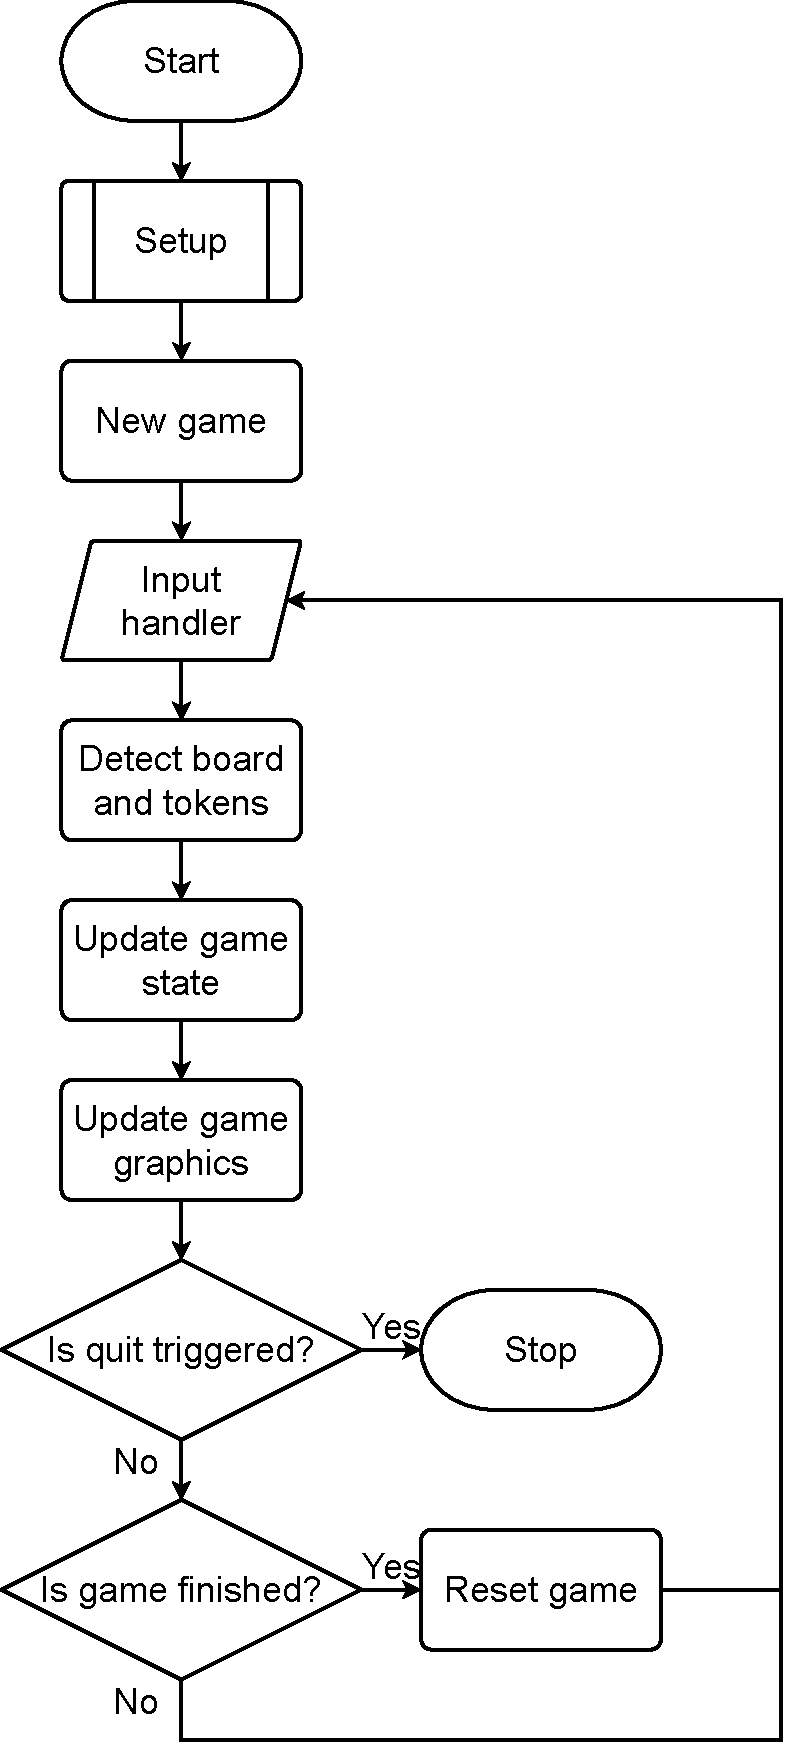
\includegraphics[width=0.55\textwidth]{images/figures/fig6a}
        \caption{Main Flowchart}
        \label{fig:maina}
    \end{subfigure}
    \caption{Main Program Flowchart}
    \label{fig:main}
\end{figure}
\begin{figure}[H]
    \ContinuedFloat
    \begin{subfigure}{1\textwidth}
        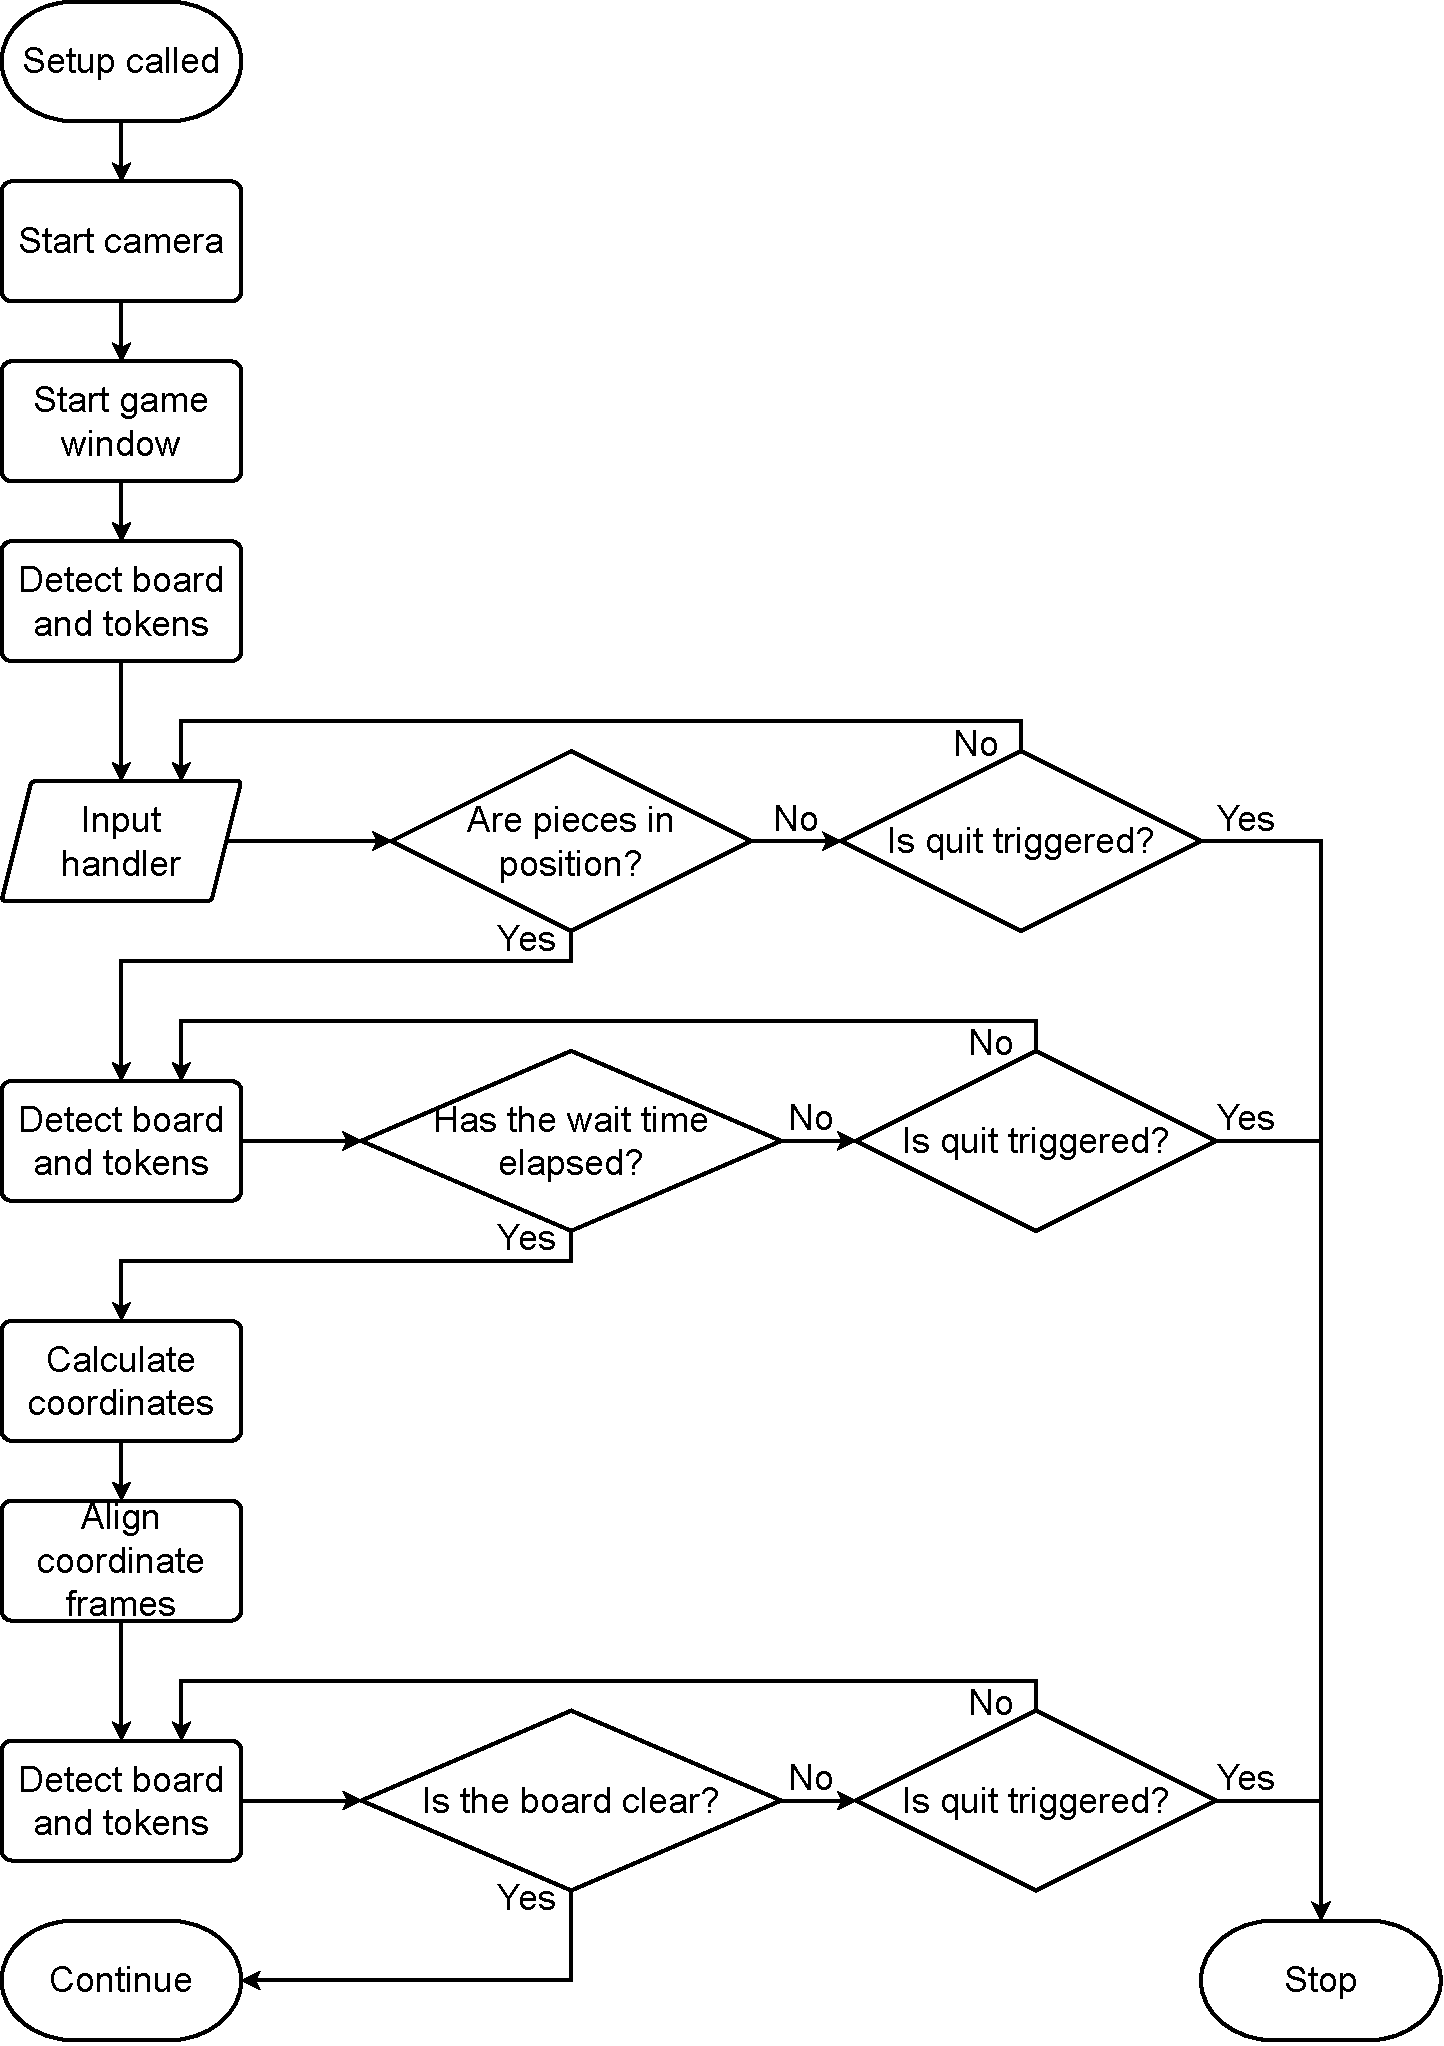
\includegraphics[width=\textwidth]{images/figures/fig6b}
        \caption{Setup flowchart}
        \label{fig:mainb}
    \end{subfigure}
    
    \caption{Main Program Setup Flowchart}
    \label{fig:main}
    %TC:endignore
\end{figure}

\subsubsection{Game Loop}
The program implements various loops which repeatedly take camera input using OpenCV, process the captured image, and display outputs via PyGame. 
The loops handle these inputs and track the state of the program. 
The main program's flow (Figure \ref{fig:maina}) invokes the setup procedure before continuing in a game loop.
Players are able to make multiple moves which update the game state.
Once the game state is updated to a terminal state, it is finished and if the quit mechanism has not been called, then then the game is reset and the players can start a new game. 

The logic for the setup procedure (Figure \ref{fig:mainb}) follows multiple stages:
\begin{enumerate}
    \item Initialise the camera
    \item Initialise the game display and create its window
    \item Calibrate token and board coordinates
    \item Clear the board of tokens
\end{enumerate}

At any point in the program, if there is a loop which waits on an action from the user or it is waiting for a defined time period, it is possible to quit and exit. This will stop all code from running and end the session. 

\subsection{Game Board Detection}
The game board is a white cardboard box, and is square in shape, measuring 24cm in width. The aim is to be able to find the bounds of the board, such that relative positions of tokens can be calculated, and a representation of the game can be projected onto the board. 

The initial approach to detect a board on the surface utilised printed QR codes as way to find the corners of a board. 
A proof of concept implementation showed that it was possible to detect printed QR codes using the camera.
However, hardware restrictions with the camera meant that it was not usable in practice. 
Due to this setback, the board is instead detected by finding contours in a threshold image of the playing surface. 

\begin{figure}[H]
    %TC:ignore
    \centering
    \begin{subfigure}{0.4\textwidth}
        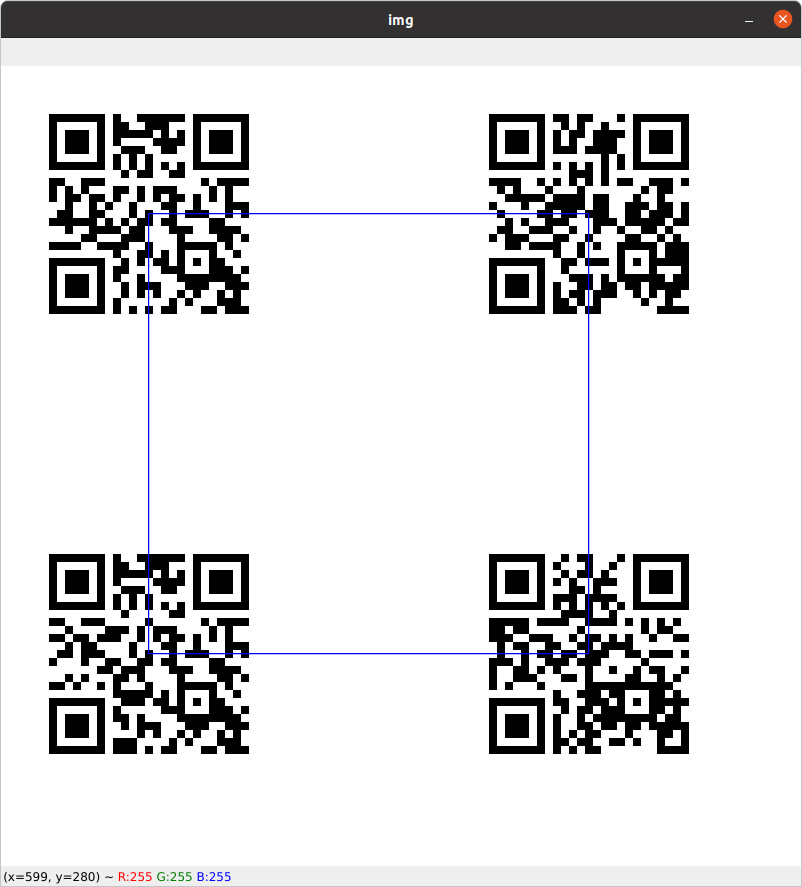
\includegraphics[width=1\textwidth]{images/figures/fig7a}
        \caption{Version 2 QR Code scanned with generated composite image file}
        \label{fig:qrcodea}
    \end{subfigure}
    \begin{subfigure}{0.4\textwidth}
        
\includegraphics[width=1\textwidth]{images/figures/fig7b}
        \caption{Version 2 QR Code detected at distance of 65cm from the camera}
        \label{fig:qrcodeb}
    \end{subfigure}
    \begin{subfigure}{0.4\textwidth}
        
\includegraphics[width=1\textwidth]{images/figures/fig7c}
        \caption{Version 2 QR Code not detectable at distance of 1.25m from the camera}
        \label{fig:qrcodec}
    \end{subfigure}
    \begin{subfigure}{0.4\textwidth}
        
\includegraphics[width=1\textwidth]{images/figures/fig7d}
        \caption{Version 1 QR Code not detectable at distance of 1.25m from the camera}
        \label{fig:qrcoded}
    \end{subfigure}
    \caption{QR Codes as passed into the detection library at various distances.}
    \label{fig:qrcode}
    %TC:endignore
\end{figure}

\subsubsection{QR Code Scanning}
This initial approach follows the process which was designed in Figure \ref{fig:qrcode} on page \pageref{fig:qrcode}. 
The implementing this is documented as a prototype in \\\texttt{prototypes/playing-surface-board-detection}.
The algorithm operates inside a infinite loop which has these steps: 
\begin{enumerate}
    \item Read image and capture still frame
    \item Crop image to the playing area by scaling by a scale factor and cropping. The scale factor depends on the local setup.
    \item Scan image for QR codes. This uses the \texttt{QRCodeDetector} class in OpenCV, detecting and decoding multiple codes in a single image.
    \item Decode and interpret the data encoded in the QR code.
    \item For the purposes of the prototype proof-of-concept, draw bounding boxes around the QR code at the coordinates found from detection.
\end{enumerate}

QR codes were initially chosen as they could encode data, meaning that each corner of the board could use a different tag. 
This would be useful as the orientation of the board could be determined, regardless of the rotation of the board about the camera's direction of gaze.
The second reason would be to distinguish between different areas on the playing surface. 
For example it may be possible to implement games with multiple boards, or ones which may involve a dice tray - which could expand on the computer-vision techniques this model utilises. 
However, it would become evident that the QR codes would not work so this idea was not explored. 

To test whether QR codes would be usable, the code initially encoded JSON data, where the \texttt{tag\_id} is "\texttt{board}" for the initial test and the anchors were "\texttt{tl}", "\texttt{tr}", "\texttt{bl}", and "\texttt{br}" for each of the top/bottom and left/right corners of the board: 
\begin{verbatim}
    { "id": <tag_id>, "anchor": <tag_anchor> }
\end{verbatim}
Using the \texttt{qrcode} library in Python, the smallest version available to generate these QR codes was a 25x25 grid (version 2). 
Choosing lowest error correction level, L, allowed for 7\% of errors in 47 alphanumeric characters.  
This was the smallest size possible size which could encode the JSON data which was 28 characters in length.

With the JSON encoded codes, it was possible to find and tag the codes when the generated image files are used as the image input (Figure \ref{fig:qrcodea}).
However, it was only possible to consistently detect the code at a short distance from the camera. 
The codes became consistently detected at 65cm from the camera (Figure \ref{fig:qrcodeb}), which would not be suitable for an application where players group around the table. 
At distances above 65cm, detail was lost in the image, and the code could not be read. 

In addition to the detection distance, at short distances, the QR codes were not able to be consistently detected in each frame. 
This meant that in many frames, there would not be any detected code in the image, even though the image would not appear to change visually. 
This was resolved by introducing a persistent data structure outside of the loop to handle updates to the point coordinates. 
In this case, a Python dictionary was used as it was possible to use the \texttt{tag\_anchor} value as a unique key.

To attempt to resolve the distance issue, a smaller QR code was generated. 
The version 1 QR code is the smallest possible code, and when using the lowest error correction level, there is a limit of 25 characters. 
The two sets codes are printed at the same size, which means the modules in the QR code are larger in Figure \ref{fig:qrcoded}. 
These version 1 codes were encoded with 1-2 arbitrary alphanumeric characters.
This was still unsuccessful, which prompted a change in approach. 

\paragraph{Limitations in Hardware.} In order for this project to be accessible, a reasonably priced camera was chosen which could perform at 1080p. 
Webcams are usually designed to capture an image of a person at a desk, and not for capturing fine details at a longer distance that it is designed for. 
This meant that there are few pixels which included the QR code in the captured image, which causes a heavily aliased and erroneous code, as seen in Figures \ref{fig:qrcodec} and \ref{fig:qrcoded}.

\begin{figure}[H]
    %TC:ignore
    \centering
    \begin{subfigure}{0.4\textwidth}
        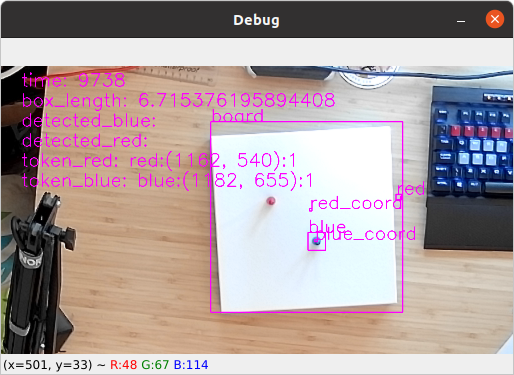
\includegraphics[width=1\textwidth]{images/figures/fig8a}
        \caption{Original captured image with labelled boards and tokens}
        \label{fig:debuga}
    \end{subfigure}
    \begin{subfigure}{0.4\textwidth}
        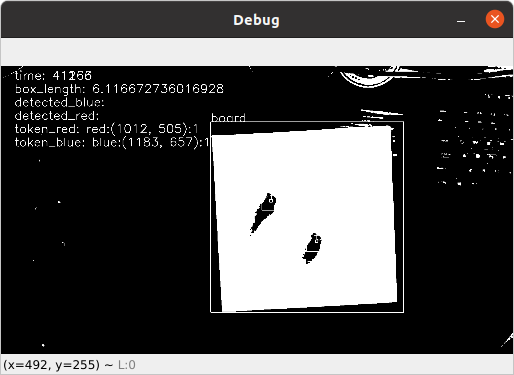
\includegraphics[width=1\textwidth]{images/figures/fig8b}
        \caption{Binary threshold of 230 applied to original captured image}
        \label{fig:debugb}
    \end{subfigure}
    \begin{subfigure}{0.4\textwidth}
        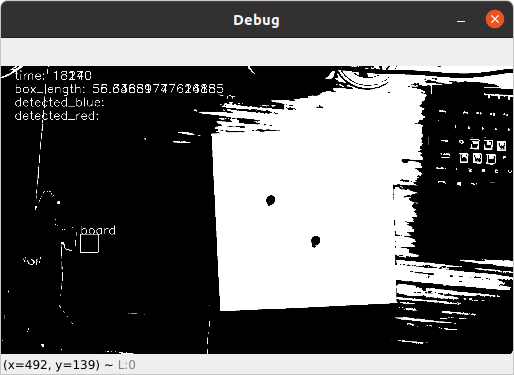
\includegraphics[width=1\textwidth]{images/figures/fig8c}
        \caption{Binary threshold of 190 applied to original captured image}
        \label{fig:debugc}
    \end{subfigure}
    \caption{Debug windows with labelled board and tokens}
    \label{fig:debug}
    %TC:endignore
\end{figure}

\subsubsection{Threshold Based Contours}
An alternative and more straightforward approach is to find the boundaries of the board based on its colour. 
The code for this algorithm is found in \\
\texttt{src/client/utils/detection/board}.
A class is created to instantiate a detection object, which can be accessed throughout the main game loop.
The process to find the boundaries relies on a variable threshold value set in the configuration files:
\begin{enumerate}
    \item A threshold value (0-255) is set in the configuration files. 
    \item Image is captured from the camera, which is passed to the detection class
    \item The source image is converted to grey scale, so there is only one colour channel
    \item The grey scale image is converted to a binary black/white image based on the threshold (Figure \ref{fig:debugb}
    \item Contours are found within the threshold converted image
    \item Contours are converted to a list of points
    \item The lists of points are checked for squareness and the largest square is assumed to be the board
\end{enumerate}

The grey scale image is an intermediate step to converting to a binary black and white image. 
This is done so it averages the colour channels, so the threshold is based on single colour channel values. 
The value of the threshold can vary a lot by the environment in which it is set up. 
During development the value has ranged between 200 and 230, but a change in 10 could make a lot of difference to how well the contour finding function operates. 
This variance is caused mainly by natural light and the reactance of the playing surface.
The natural environment has been a significant challenge in developing the board detection algorithm, which can be seen in Figures \ref{fig:debugb} and \ref{fig:debugc}.
The threshold images were taken at the same time (where the lighting conditions are identical), but the threshold value varied by 40.
In this case the value of 230 worked well, but when the 190 threshold was applied, too much reflected light from the desk surface was reflected, meaning it was not possible to find the edges of a square. 

The contours of the shape find a white object in a black background image, providing points along the boundary of the shape. 
In this application the board is the white object in the threshold image. 
Contours are found using OpenCV's \texttt{findContours} function, using a simple chain approximation method\footnote{\url{https://docs.opencv.org/4.x/d4/d73/tutorial_py_contours_begin.html}}. 
Instead of finding all the points along the boundary, the contour is compressed to remove redundant points along the same boundary. 
In this case, the object is square so it is beneficial to use a simple approximation to remove points along the edges. 
This saves on computation and memory as only the four vertices of the board are stored. 
These values are them used to derive a bounding box of the board area, where tokens can be searched.

Contour finding works much better if there is a contrasting background below the board. 
This algorithm also works well where the board has a contrasting edge colour. 
The design decision was chosen not to require this as the model should remain versatile, although performance would be improved if players chose to use this style of setup. 

\paragraph{Smoothing Buffer.} Overall, this approach performed a lot better than using QR codes. 
Finding the board was more consistent at farther distances from the camera as it did not rely on fine details in pixels. 
However, the same issues still applied with inconsistency between frames. 
The camera image was reasonable noisy as lighter areas of the image were near the threshold. 
This meant there were many areas which were candidates for being a board. 
For this reason, the search area was limited to a zoomed-in area of the camera's image and only the largest object was assumed to be the board. 
This reduced false positives in detecting the board object, but the contours jittered between frames, as they moved slightly and changed in size. 

To reduce the impact of jitter in the board size, a buffer was implemented to calculate the average position of the board. 
Each frame where a board's boundaries are found, they are added to the buffer. 
If the board is not found in the image then the buffer does not update. 
This buffer object stores the previous 15 board coordinates, and provides the average coordinate every frame. 
This number was chosen as it seemed to work best during testing: it did not jitter too much, but updated reasonably quickly if the board was moved. 

While the smoothing buffer helped to make the board's position a less erratic, it did allow the board position to deviate. 
If the board itself was not found in a pass through the board detection algorithm, then there may be false positives in other locations in the frame. 
Since these are the added to the buffer, the size and position of the board would deviate over a few seconds to be incorrect.
During development, this kind of error usually made the board bounds smaller and move towards the lighter areas of the frame. 
This issue would be partially resolved by constraining the buffer to only accept values which are close to the true size of the board. 

\subsubsection{Debug Tool}
As stated previously, the threshold for light varied in a problematic way. 
During development of proof-of-concept prototypes, this was not an issue as the OpenCV \texttt{imshow} function was relied on to display various processed images. 
However, in the main program, this was not practical as the PyGame window would need to be full screen to be projected onto the board. 

Therefore in order to aid development, a debug tool was implemented which displays the camera feed input over the PyGame window (Figure \ref{fig:debug}). 
In each of the loops where an image is captured, the captured image is also passed to the debug tool which displays the frame.
This gives a live view of the what the camera has vision of, and what the images being processed look like.
The image was annotated with bounding boxes and labels around where identified objects are located, as well as listing values of prescribed variables such as time and coordinates. 

This tool guided resolving issues of board and token placement. 
In particular it was vital in the development and debugging of threshold values in board detection. 
It was also very useful in finding positions of tokens in their detection.

\begin{figure}[h]
    %TC:ignore
    \centering
    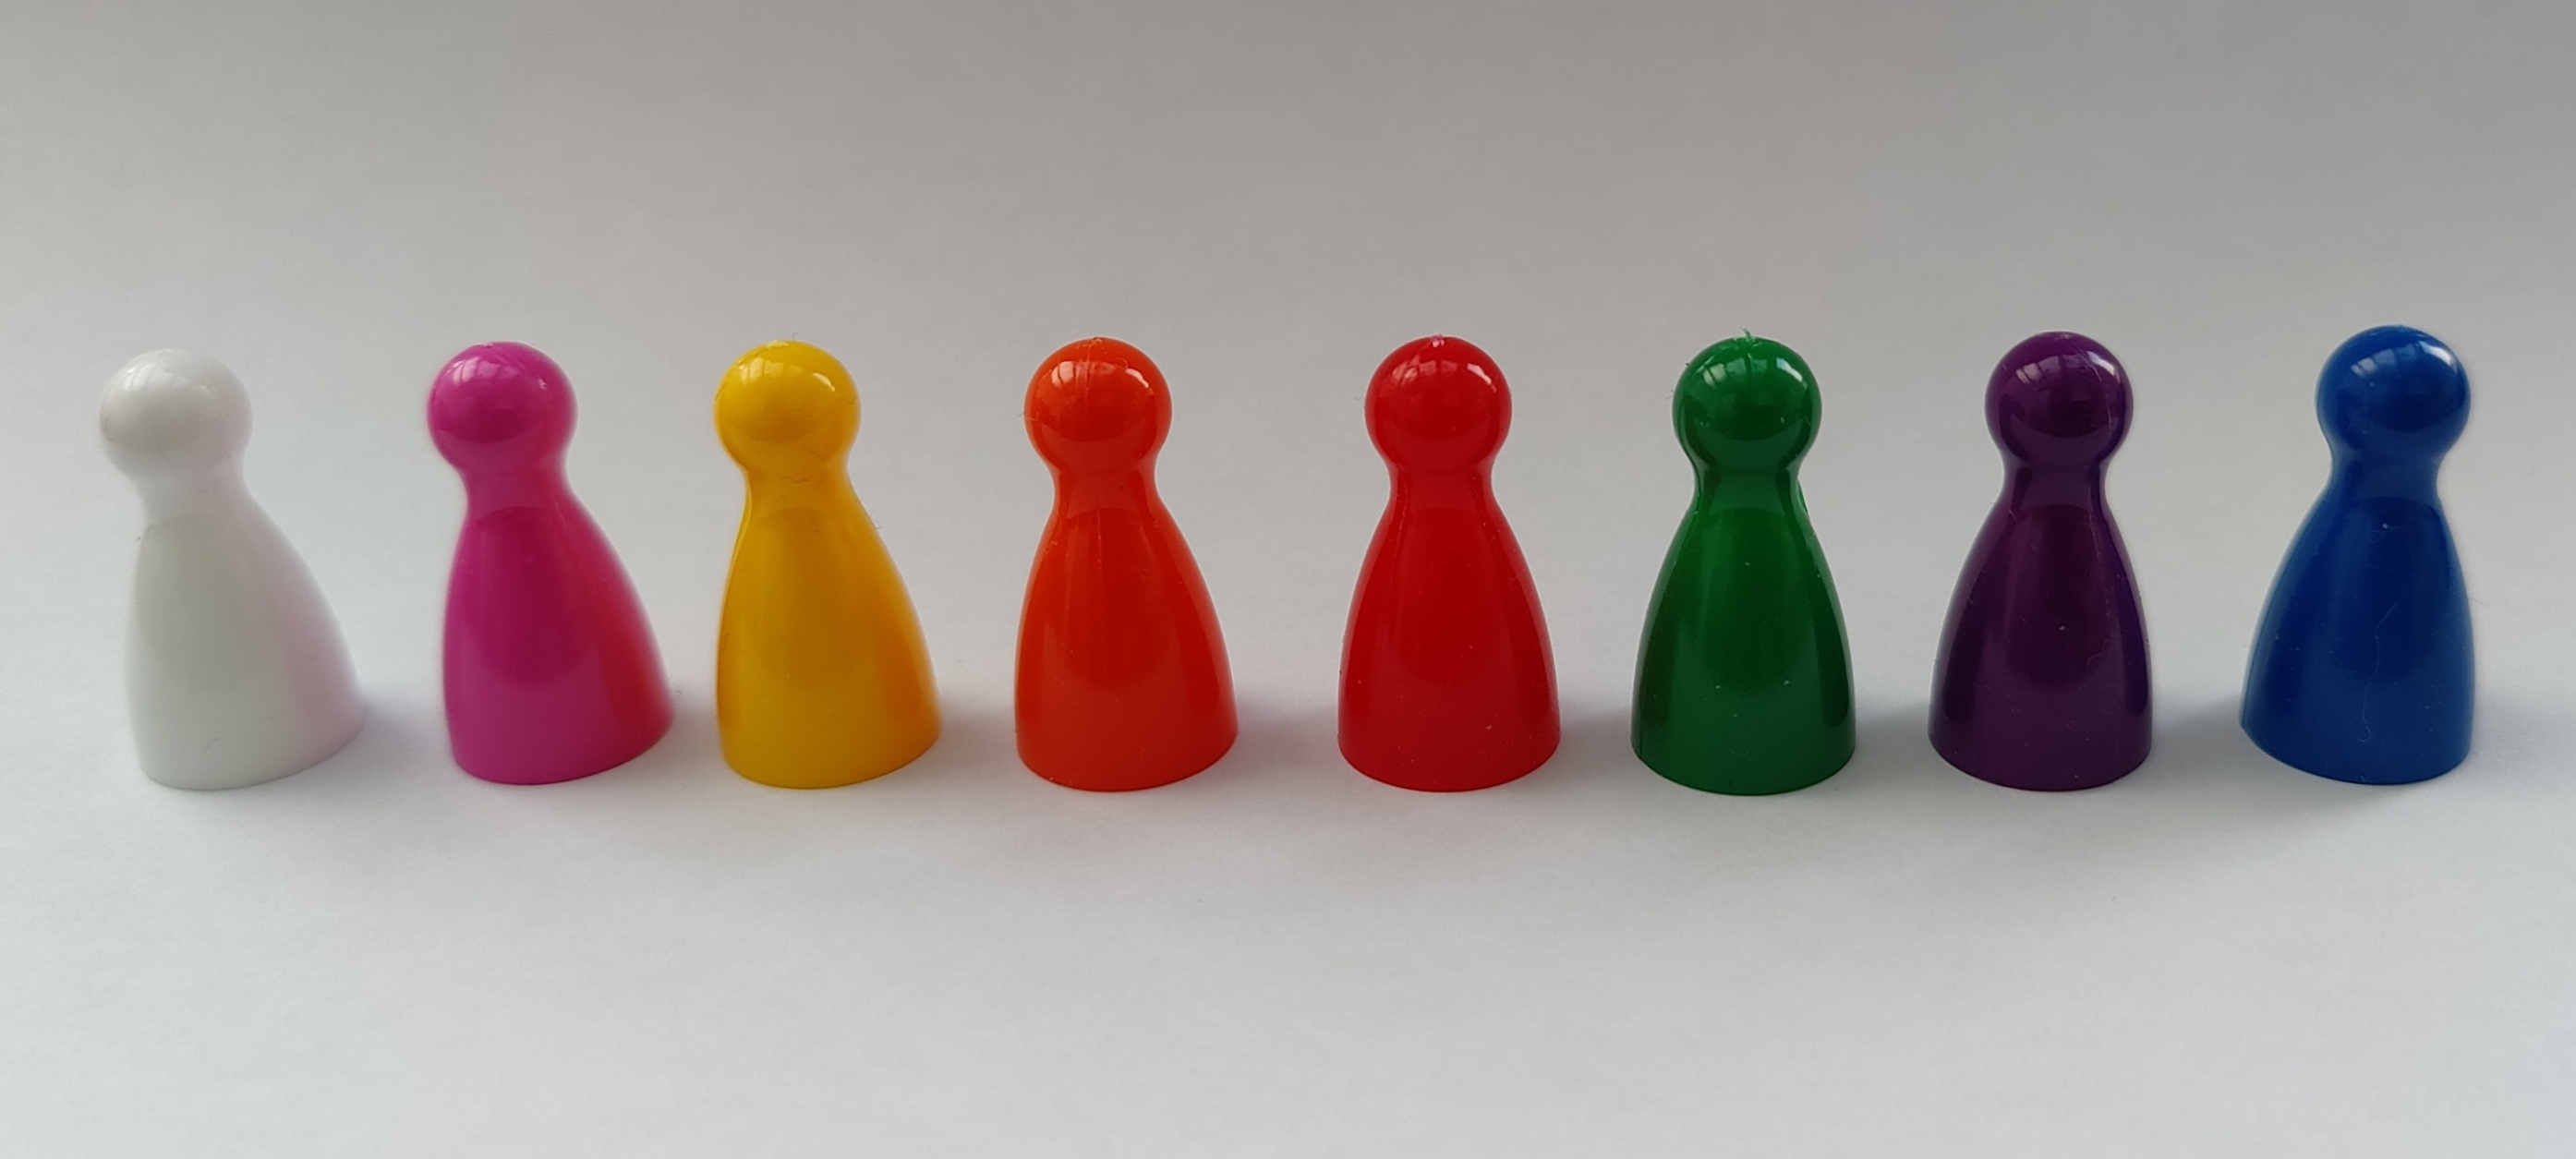
\includegraphics[width=0.8\textwidth]{images/figures/fig9}
    \caption{Game Token Pieces}
    \label{fig:tokens}
    %TC:endignore
\end{figure}

\begin{figure}[H]
    %TC:ignore
    \centering
    \begin{subfigure}{0.2\textwidth}
        
\includegraphics[width=1\textwidth]{images/figures/fig10a}
        \caption{White Token}
        \label{fig:tokencolora}
    \end{subfigure}
    \begin{subfigure}{0.2\textwidth}
        
\includegraphics[width=1\textwidth]{images/figures/fig10b}
        \caption{Pink Token}
        \label{fig:tokencolorb}
    \end{subfigure}
    \begin{subfigure}{0.2\textwidth}
        
\includegraphics[width=1\textwidth]{images/figures/fig10c}
        \caption{Yellow Token}
        \label{fig:tokencolorc}
    \end{subfigure}
    \begin{subfigure}{0.2\textwidth}
        
\includegraphics[width=1\textwidth]{images/figures/fig10d}
        \caption{Orange Token}
        \label{fig:tokencolord}
    \end{subfigure}
    \begin{subfigure}{0.2\textwidth}
        
\includegraphics[width=1\textwidth]{images/figures/fig10e}
        \caption{Red Token}
        \label{fig:tokencolore}
    \end{subfigure}
    \begin{subfigure}{0.2\textwidth}
        
\includegraphics[width=1\textwidth]{images/figures/fig10f}
        \caption{Green Token}
        \label{fig:tokencolorf}
    \end{subfigure}
    \begin{subfigure}{0.2\textwidth}
        
\includegraphics[width=1\textwidth]{images/figures/fig10g}
        \caption{Purple Token}
        \label{fig:tokencolorg}
    \end{subfigure}
    \begin{subfigure}{0.2\textwidth}
        
\includegraphics[width=1\textwidth]{images/figures/fig10h}
        \caption{Blue Token}
        \label{fig:tokencolorh}
    \end{subfigure}
    \caption{Coloured Tokens as visible to the camera}
    \label{fig:tokencolor}
    %TC:endignore
\end{figure}

\subsection{Player Token Detection}
Player tokens consisted of 8 different colours: white, pink, yellow, orange, red, green, purple, and blue (Figure \ref{fig:tokens}). 
It was determined that it was not necessary to have eight colours implemented in this game, so the set was initially reduced to four colours.
This was done after analysing images of the tokens on the board surface. 
With a camera close to the pieces the colour accuracy is reasonable, as seen in Figure \ref{fig:tokens}.
When the camera is distant, the colour is significantly different, as seen when comparing Figure \ref{fig:tokens} and \ref{fig:tokencolor}. 
The white, pink, and yellow tokens are very similar in colour to the background. 
This would make it harder to distinguish the colour of these tokens. 
In addition, the orange token is very similar in colour to the red token, so it was also discarded. 
Therefore four tokens remain in use: red, green, purple, and blue. 
 
The board was detected using thresholds to identify shape. 
In Figure \ref{fig:debugb} and \ref{fig:debugc} it is possible to see that shadows are cast by tokens. 
This means that tokens can vary in shape and it may be difficult to correctly identify tokens from other objects. 
Therefore Haar Cascade Classifiers were trialled as a proof-of-concept to detect the tokens. 

Cascade Classifiers are feature based classifiers which are machine-learning based. 
A cascade function is training using positive and negative sample images. 
Features where there are edges, lines, or rectangles are found in the positive sample images. 
OpenCV provides classifier training tools which ingest data collected\footnote{\url{https://docs.opencv.org/3.4/db/d28/tutorial_cascade_classifier.html}}.

\begin{figure}[h]
    %TC:ignore
    \centering
    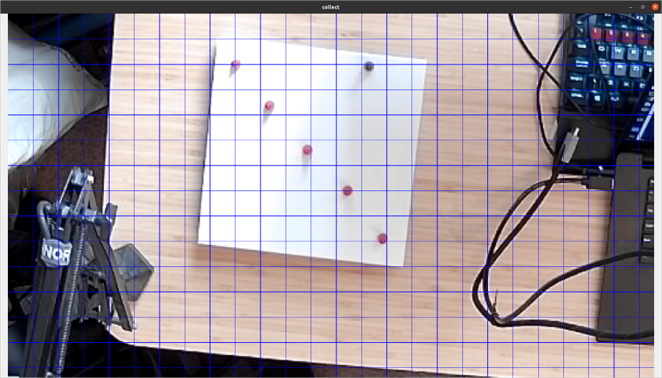
\includegraphics[width=0.8\textwidth]{images/figures/fig11}
    \caption{Data Collection Tool}
    \label{fig:collect}
    %TC:endignore
\end{figure}

\subsubsection{Data Collection}
The data to train and test on is quite unique in this project, so data must be collected manually. 
The positive images would include a token on the background, while the negative images should only include sections of the board. 
A utility tool helps with data collection where a point and click interface aids with collecting many sample images in a short space of time. 
Figure \ref{fig:collect} shows the tool which was created, and it can be found in\\
\texttt{prototypes/game-piece-detection/src/training/collect/\\collect\_dataset.py}. 
Clicking on a token creates a 50x50 pixel cropped image around the cursor point. 
This image is saved into the data directory, and can be found in Appendix \ref{app:data}.
A blue 50x50 pixel grid is used as a guide to compare the size of the saved image. 

Creating this tool was very useful as it meant that data collection was a quick and efficient process. 
Through using this tool, a total of 415 positive samples and 145 negative samples were taken and used in the model training.
Samples varied in distance from the camera, as well as being in light or shadow, and casting their own shadows. 
Figure \ref{fig:collect} shows six tokens in different positions on the board, which have different lighting conditions. 
Collecting a range of images means the model will be better trained to identify the features of a token in different conditions.
The style of the sample files is identical to the images in Figure \ref{fig:tokencolor}.

\paragraph{Positive Samples.} Samples were collected for each of the four colours, with approximately 100 samples each. 
Almost all positive samples included a shadow. 
This is because the samples were taken during the day and nearby a window. 

\paragraph{Negative Samples.} In total 600 samples were taken, however only 145 samples were used in the final model. 
The samples used were of the board and its edges. 
Samples which included sections of other items in the image were not used. 
This is shown in Figure \ref{fig:negatives}.

\begin{figure}[h]
    %TC:ignore
    \centering
    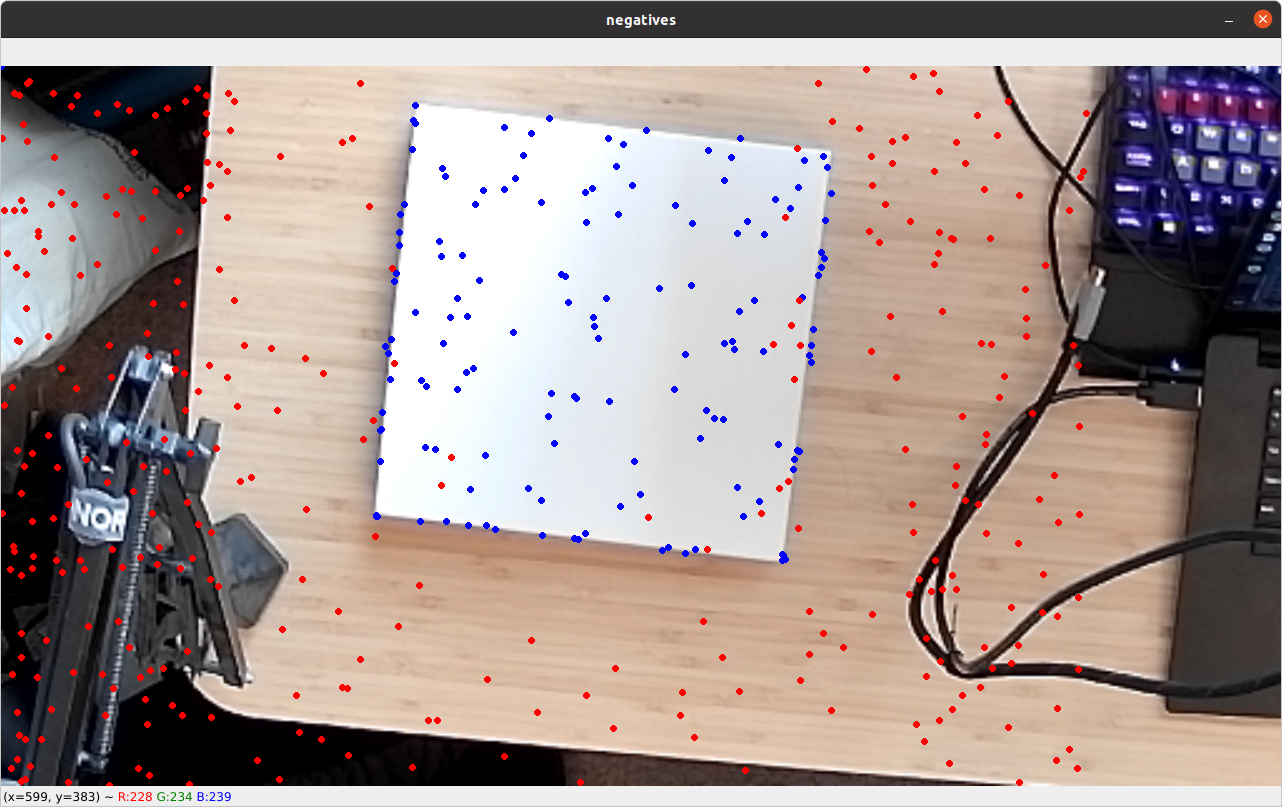
\includegraphics[width=0.8\textwidth]{images/figures/fig12}
    \caption[Distribution of accepted negative samples and rejected samples]{Distribution of accepted negative samples (blue) and rejected samples (red)}
    \label{fig:negatives}
    %TC:endignore
\end{figure}

\subsubsection{Experimental Models}
After sample collection, the data was used to train a model and tested. 
Since the data is limited to only tokens, there are very few features to distinguish from. 
In comparison, a human face will have many edge and line features, while the token is essentially a round circle on the board with a shadow. In combination with the low resolution images, being only 50 pixels wide, the models required fine tuning to reduce false positives.  
The results of these initial experimental models and final model are in Appendix \ref{app:tokens}. The models themselves can be found in Appendix \ref{app:data}.

\paragraph{Initial Attempts.} In the first few experiments at training the model, only the red positives were used, along with the 145 negative samples. 
The first attempt produced a satisfactory result, and correctly identifies tokens on a board. 
There were however significant false positives around the edge of the desk and where the board casts shadows. The model also produced a lot of lag, which made it unsuitable for real time token detection. 

The second and third attempts were less successful where the parameters were altered.
The second experiment attempts to use LBP classifiers instead of Haar classifiers, while also increasing the proportion of positive and negative samples used to train. 
Training used 90 positive samples and 130 negative samples in this model, instead of the 75 positives and 100 negatives out of 100 and 145 samples in total respectively. 
Local Binary Patterns generally are faster, but are less accurate. 
This reduced the long processing time to identify objects in the first model.
This is shown in the results as it increases the number of false positives, especially around the desk surface. 
This model also trained for a significantly longer time; where the first model trained for only 1 second before halting, this one trained for 5 minutes. 

The third experiment increased the number of cascade stages which the training ran for. The data was also expanded to include all 600 background samples, while still only including the red token samples. 
This again increased false positives.

\paragraph{Combined positive samples.} Cascades look at the black/white features of the image, so colour detail is lost. 
Combining the whole positive data set provided more data to train with. 
In order to adapt the original segregated data into a single list of annotations, the script at \\
\texttt{prototypes/game-piece-detection/src/training/collect/\\create\_combined\_positive\_set.py} was created. 
In these experiments, the whole negative data set was still included which continued to produce many false positives. 
Removing the non-game board samples improved results. 
The sample locations for the included negative images is shown in Figure \ref{fig:negatives}.
Since the LBP classifier was less accurate, these later experiements returned to using the Haar cascade model to train. 

\paragraph{Final Result.} The final model training for 17 seconds. 
The number of positives used to train this model was reduced to 100 of the 400 samples, while the negative background samples used 100 of the 145 samples to train. 
This model resulted in the least false positives so was chosen as the final model. 

\subsubsection{Implementation}
\texttt{src/client/utils/detection/tokens.py} implements the cascade model to detect tokens. 
The fact that even with the best model found through experiments still included false positives reinforced the earlier decision to reduce the search area for tokens to the board. 
This will mean that no false positives outside the board will be detected, but it also has the benefit of reducing computation by not needing to compute objects outside of the board. 
The process for identifying tokens is quite straightforward, as the board image is cropped and the classifier is applied to the image. 
This produces bounding boxes for tokens, so new \texttt{Token} objects can be instantiated.

Tokens also implement a smoothing buffer, in the same way as used for the board. 
The cascade classifier also does not consistently detect the tokens, so there are some frames where no tokens are found. 
Additionally, the source data included images of the tokens taken at different heights from the camera. 
This means that some tokens in the data set appear smaller than others, so the bounding boxes of detected tokens also vary in size. 
For this reason the buffer averages the position coordinates of the tokens as well as the size. 

\begin{figure}[h]
    %TC:ignore
    \centering
    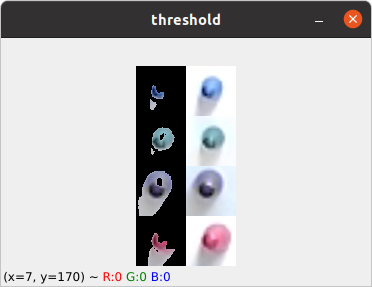
\includegraphics[width=0.6\textwidth]{images/figures/fig13}
    \caption{Token threshold value utility tool}
    \label{fig:threshold}
    %TC:endignore
\end{figure}

\begin{figure}[h]
    %TC:ignore
    \centering
    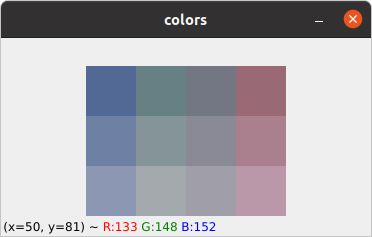
\includegraphics[width=0.6\textwidth]{images/figures/fig14}
    \caption{Maximum, mean, and minimum RGB values for colour of tokens}
    \label{fig:tokenrgb}
    %TC:endignore
\end{figure}

\subsubsection{Token Colour Classification}
Token detection is able to identify position on the board, but is not able to differentiate between colours of tokens. Therefore, colour must be classified pragmatically. 

As previously discussed, Figures \ref{app:tokens} and \ref{fig:tokencolor} show that the colours of tokens differ from real life and how the camera views it. 
In order to calculate the colour of a token, the background must first be filtered out. 
This step can be done in a similar way to threshold application in the board detection algorithm. 
However, in this case the threshold value must be more finely tuned. 
Another utility tool was created to determine the best threshold value of the data set. 
This tool can be found in \texttt{prototypes/game-piece-detection/detect\_color.py}. 
The \texttt{find\_threshold} function was used to find that the best value for filtering out the background in the data was 200/255. 

After the background is filtered out, the non-black pixels are either token colour or shadow (Figure \ref{fig:threshold}). 
The non-black pixels for all images in the dataset are iterated through, finding the highest, lowest, and mean RGB values (Figure \ref{fig:tokenrgb}). 
The mean value is used as it is a simple way to find the colour of the token. It is possible to use the most dominant colour in an image, but this had no effect on the actual outcome of this process. 
Simply stated, the dominant colour, and mean colour are essentially identical in this application. 
These define the RGB values for each colour class. 

To determine the colour of a detected token, the process is identical.
A RGB value for that token is found by averaging the non-black pixels after it is passed through the threshold filter. 
The colour classification is then determined by the lowest Euclidean distance between the detected RGB colour, and the mean RGB value for each token colour. 

\begin{figure}[h]
    %TC:ignore
    \centering
    \begin{tabular}{ c c c c }
        Token Colour & Red & Green & Blue \\
        Blue & 110 & 128 & 163 \\
        Green & 133 & 148 & 152 \\
        Purple & 137 & 138 & 150 \\
        Red & 170 & 128 & 143
    \end{tabular}
    \caption{Token Colours and found RGB values}
    \label{fig:tokenrgbtable}
    %TC:endignore
\end{figure}
\begin{figure}[h]
    %TC:ignore
    \centering
    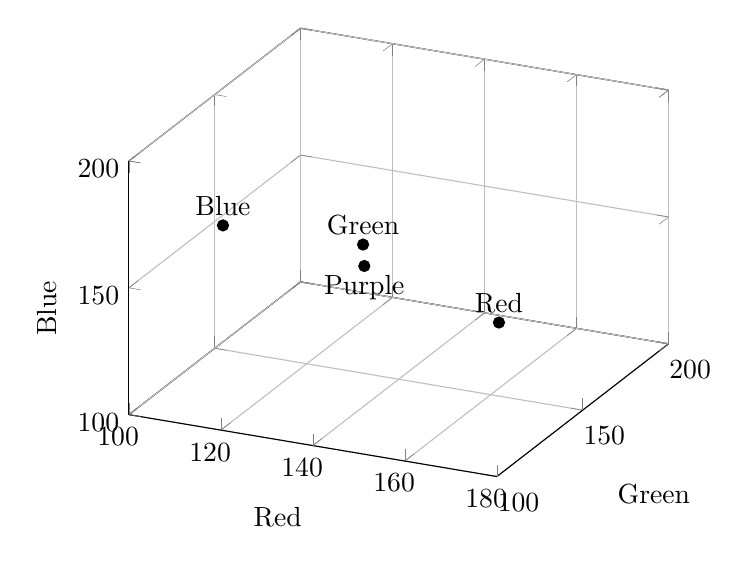
\begin{tikzpicture}
        \begin{axis}[xmin=100,xmax=180,ymin=100,ymax=200,zmin=100, zmax=200,grid,xlabel={Red},ylabel={Green},zlabel={Blue}]
            \addplot3[mark=*, nodes near coords=Blue] coordinates {(110, 128, 163)};
            \addplot3[mark=*, nodes near coords=Green] coordinates {(133, 148, 152)};
            \addplot3[mark=*, node near coords style={yshift=-0.55cm},nodes near coords=Purple] coordinates {(137, 138, 150)};
            \addplot3[mark=*, nodes near coords=Red] coordinates {(170, 128, 143)};
        \end{axis}
    \end{tikzpicture}
    \caption{Token Colours as 3D vector}
    \label{fig:tokenrgbplot}
    %TC:endignore
\end{figure}

In Figure \ref{fig:tokenrgbplot}, it is evident that the Green and Purple coloured tokens are very near eachother.
In fact the Euclidean distance between the two colours is $10.95$. 
This reinforces the observation that during development, green and purple tokens were incorrectly classified. This is contrast by the distance between the red and blue colours: $63.25$.
This increased distance is better for colour classification as the noise the camera introduces would not impact the classification as much. 

This leads to the decision to remove a further two token colours: green and purple, leaving only red and blue. 
This change means that classification of colours is more consistent as they must choose between either red or blue.

\begin{figure}[H]
    %TC:ignore
    \centering
    \begin{subfigure}{0.65\textwidth}
        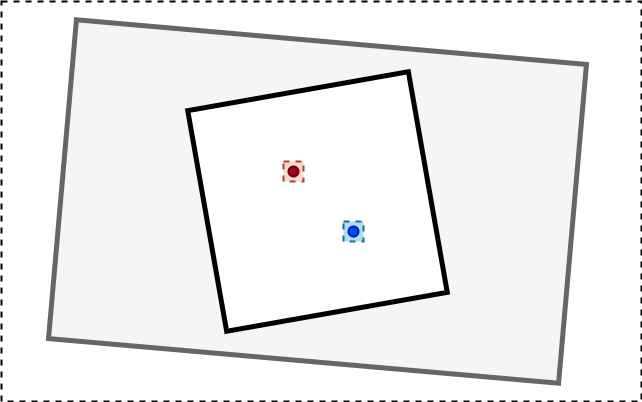
\includegraphics[width=1\textwidth]{images/figures/fig15a}
        \caption{Composite projection and camera view}
        \label{fig:calibrationa}
    \end{subfigure}
    \begin{subfigure}{0.65\textwidth}
        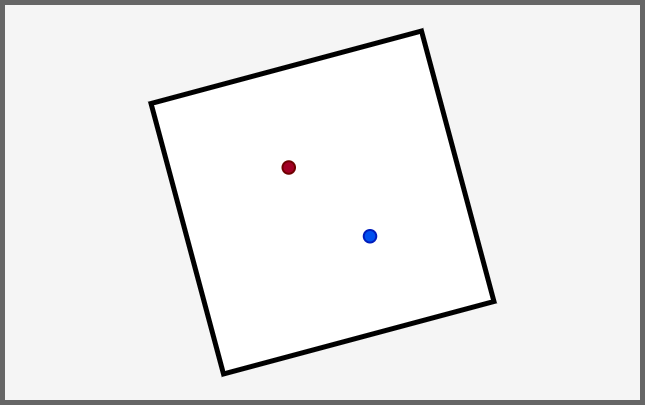
\includegraphics[width=1\textwidth]{images/figures/fig15b}
        \caption{Camera's view of tokens placed in a known location}
        \label{fig:calibrationb}
    \end{subfigure}
    \begin{subfigure}{0.65\textwidth}
        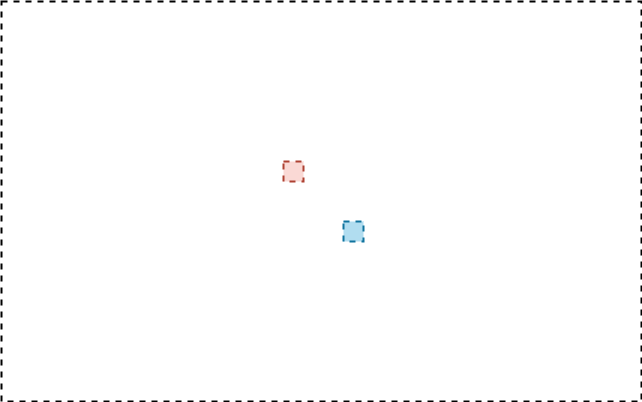
\includegraphics[width=1\textwidth]{images/figures/fig15c}
        \caption{Projection of known location onto playing surface}
        \label{fig:calibrationc}
    \end{subfigure}
    \caption{Composite, camera view, and projection of calibration process}
    \label{fig:calibration}
    %TC:endignore
\end{figure}

\subsection{Calibration}
The board detection algorithm provides a bounding box around the physical board in the camera's coordinate frame. 
However, in order to project onto the board, the board's position must be known in the projector's coordinate frame. 
Therefore, aligning the camera and projector coordinates is required to be able to project a game state onto the board. 
Fortunately, basic matrix transformations on coordinates provide the required coordinates. 
In order to do this, fixed points in both coordinate frames must be known. 
The code for this process is in\\\texttt{src/client/utils/calibration/calibration.py}

\textbf{1. Two differing coloured squares are projected onto the playing-surface.} 
A small red square and small blue square is projected onto the playing surface (Figure \ref{fig:calibrationc}). 
It is placed into a known location relative to the centre of the PyGame window and projector's coordinate frame. 
These are the target points of the transformations which will be applied.

\textbf{2. The player is asked to place the corresponding coloured token on the coloured square.} 
This enforces the tokens to be in a precise location in the physical world, i.e. in the same place as the coloured squares. 
The setup will look like Figure \ref{fig:calibrationa}, where the solid lines are what the camera captures, and the dotted lines are the projected graphics. 
The coordinates of the tokens is detected in the camera's coordinate frame (Figure \ref{fig:calibrationb}). 
These are the coordinates which will need to be transformed into the positions on the projection.

\textbf{3. The player is asked to press space once the tokens are placed.} 
This is so the calibration process only continues once the player has placed the pieces correctly.

\textbf{4. The calibration process waits for 10 seconds.} 
The token coordinates are calculated from the average buffer, so the wait time allows the coordinate values to average and converge on the point of the token. 
This should remove any errors caused by any token detection false positives. 

\textbf{5. The coordinates are aligned with matrix transformations}. 

\textbf{6. The player is asked to remove the two tokens from the board.} 
This ensures the board is empty before the game starts, so that it does not immediately recognise a move.

\subsubsection{Matrix Transformations}
Once the user completes calibration, four coordinates are known: the red and blue tokens in each of the camera and projector's coordinate frames. 
Differently stated, one set of matrix transformations are calculated which transforms the red camera point onto the red projector point, while also transforming the blue points in the same way. 

Each coordinate is a 2D matrix with their respective $x$ and $y$ values:
\[
C_{red}=
\begin{bmatrix}
x \\ 
y
\end{bmatrix},
C_{blue}=
\begin{bmatrix}
x \\ 
y
\end{bmatrix},
P_{red}=
\begin{bmatrix}
x \\ 
y
\end{bmatrix},
C_{blue}=
\begin{bmatrix}
x \\ 
y
\end{bmatrix}
\]

\paragraph{Transform to origin.} The transformations are done with the red camera coordinate as an anchor point. The first step is to transform the camera points towards the origin. 
\[
T_1 = -C_{red}
\]

\[
C_{red} =  
\begin{bmatrix}
0 \\ 
0
\end{bmatrix},
C_{blue} = C_{blue} + T_1
\]

\paragraph{Scale camera to projector.} Once the anchor point is at the origin, it can be scaled such that the distance between the red and blue points in the camera frame ($||C_{blue}-C_{red}||$) becomes equal to that distance in the projector frame ($||C_{blue}-C_{red}||$).
\[
s_x = \dfrac{ P_{blue,1} - P_{red,1} }{ C_{blue,1} - C_{red,1} },
s_y = \dfrac{ P_{blue,2} - P_{red,2} }{ C_{blue,1} - C_{red,2} }
\]
\[
S = 
\begin{bmatrix}
s_x & 0 \\
0 & s_y
\end{bmatrix}
\]

So, the camera points can be scaled to the projector scale.
\[
C_{red} = 
\begin{bmatrix}
0 \\
0
\end{bmatrix},
C_{blue} = S \cdot C_{blue}
\]

\paragraph{Rotate the blue camera point} such that it at is the same angle as the projector red to blue ($\dfrac{\pi}{4}$ radians anti-clockwise from the $y$-axis). The angle of rotation is the difference between the current angle to the target angle. This means the unit vector for both red-blue pairs would be the same.
\[
P_{rb} = P_{blue} - P_{red},
\theta_P = arctan2(P_{rb1}, P_{rb2})
\]
\[
C_{rb} = C_{blue} - C_{red},
\theta_C = arctan2(C_{rb1}, C_{rb2})
\]
\[
\theta_R = \theta_P - \theta_C
\]
\[
R = 
\begin{bmatrix}
cos(\theta_R) & -sin(\theta_R) \\
sin(\theta_R) & cos(\theta_R)
\end{bmatrix}
\]
\[
C_{blue} = R \cdot C_{blue}
\]

\paragraph{Translate to final position.} The final position of the red and blue camera coordinates will be on the red and blue coordinates in the projector frame.
\[
T_2 = P_{red}
\]
\[
C_{red} = P_{red},
C_{blue} = C_{blue} + T_2
\]

\paragraph{Applied to a point.} Therefore, the four transformations have been defined, and can be applied to any point in the camera coordinate frame. That is, a camera coordinate can be transformed to a point on the projector coordinate frame. If $C$ is a point in the camera coordinate frame, then $P$ is the same point in the projector coordinate frame.
\[
P = (R \cdot S \cdot (C + T_1)) + T_2
\]

\begin{figure}[H]
    %TC:ignore
    \centering
    \begin{subfigure}{0.65\textwidth}
        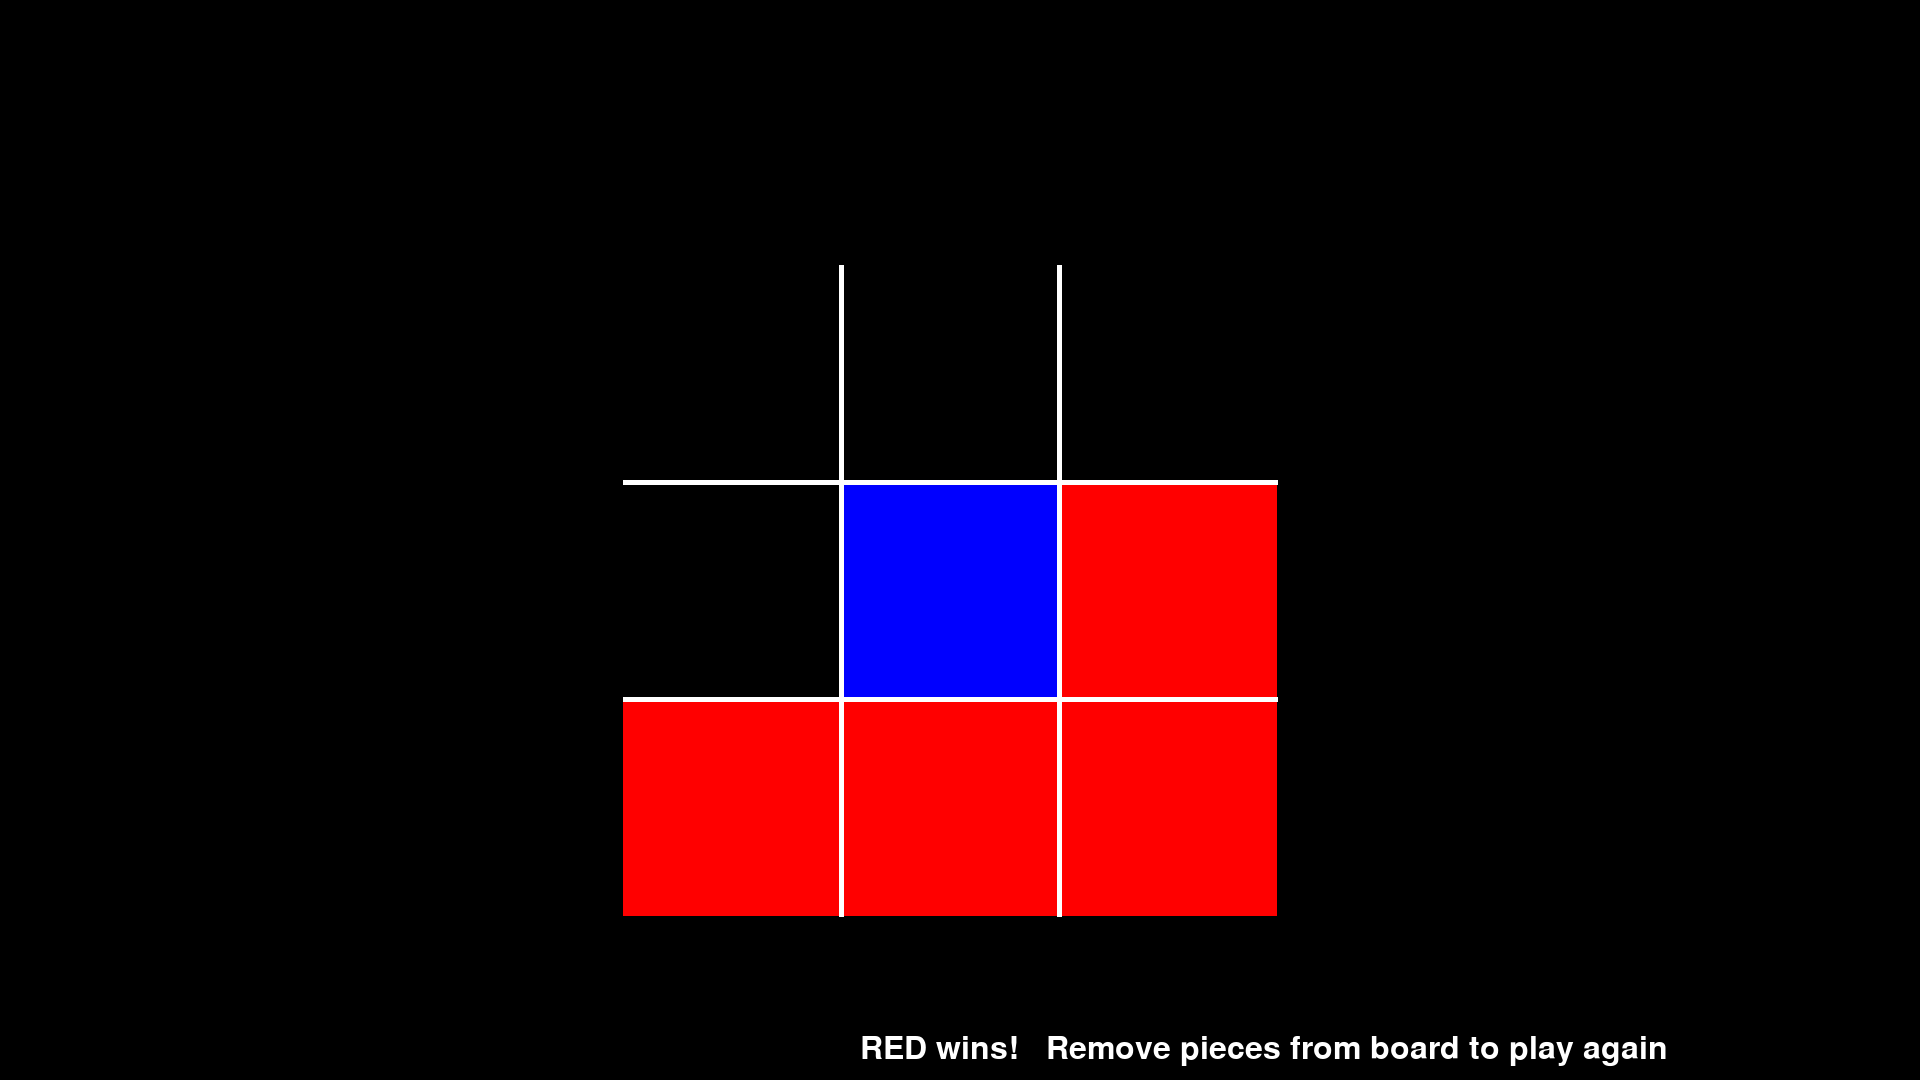
\includegraphics[width=1\textwidth]{images/figures/fig16a}
        \caption{PyGame Window showing the state of the game}
        \label{fig:tictactoea}
    \end{subfigure}
    \begin{subfigure}{0.65\textwidth}
        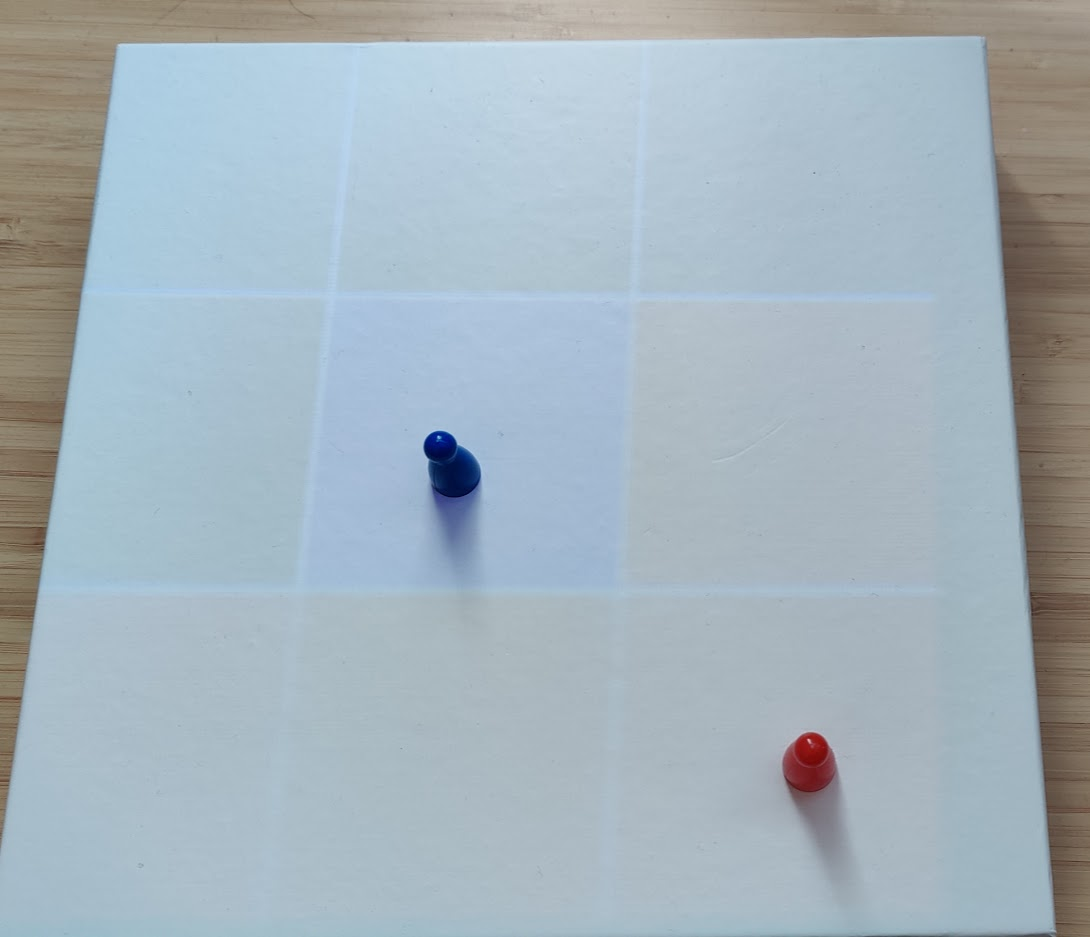
\includegraphics[width=1\textwidth]{images/figures/fig16b}
        \caption{Player's perspective of the game}
        \label{fig:tictactoeb}
    \end{subfigure}
    \caption{Example of tic-tac-toe where the red player has won}
    \label{fig:tictactoe}
    %TC:endignore
\end{figure}


\subsection{Implementing Games}
Since it's possible to transform points from the camera's coordinate frame to the projector's frame, it is possible to reflect the position of a placed token through the game state.
Tic-tac-toe is implemented as it was designed. 
Once players complete the calibration, a grid is drawn on the board.
Players are then able to place a token, which is detected and it's tic-tac-toe grid location calculated. 
The calculated grid cell is then updated to be occupied by that colour token. 

The only game logic which is implemented is the win condition. 
Once a single colour token occupies three horizontal, vertical, or diagonal grid cells, then they win. 
A message is displayed to the user that there is a winner, and they are invited to clear the board of tokens and play again.

The game was implemented in a modular way, so it is possible with minimal effort, change the implemented game. 
Token positions are passed to a \texttt{GameHandler} class, which implements the logic to convert the position into a move. 
With the move calculated, it handles updates to the game graphics through the \texttt{TicTacToeBoard} class, which extends the PyGame sprites. 

Figure \ref{fig:tictactoe} shows an example play-through where the players are free to implement their own rules. 
The image shown in Figure \ref{fig:tictactoea} is projected onto the desk surface, placing the grid the board. The cells are highlighted to show the current game state.
The red player has played four moves and won, while the blue player has only played one. 
Figure \ref{fig:tictactoeb} also highlights the issue of natural light, as the projection is not bright enough to combat the ambient conditions. 

\subsection{Configured Client}
Many of these processes rely on configured values which can easily and frequently vary. Values such as the resolution of the camera, or game window are defined and rarely change. However, other figures such as the light thresholds vary based on ambient light conditions. 

A configuration object is made available via a module import, which allows a configuration parameter file to be read and values accessible. 
Parameters are stored in a YAML file which allows for simple modifications for the players. 
The file \texttt{src/client/config.yaml} has many parameters, most notably:
\begin{itemize}
    \item Board and Token colour thresholds. These control how much light is filtered out in the board and token detection stages.
    \item Token class colour values. The actual colour of tokens may vary for players, this allows that value to change to better classify the tokens.
    \item Smoothing buffers. These allow adjustment to the lengths of the buffers.
    \item Camera and Projector resolutions. These may change depending on what peripherals are used.
\end{itemize}
This configuration file also eases development, as all of the variables can be adjusted in a single location.

\subsection{Networked Clients}
This project allows a single person or group of people to interface with a digital game. 
A feature often presented with digital games is the ability to play with others online. 
An initial proof of concept was attempted to develop a network interface which would send moves over the internet to a server. 
Unfortunately, this attempt was unsuccessful as it was not able to run smoothly and send data over a network. 

Many aspects of this project were developed with networking in mind. The source code contains a \texttt{client} directory which contains the current program's code. 
A \texttt{common} module is also available which contains utilities which would be shared or useful if a server was implemented. 

The concept of a networked client is to utilise the client-side software as a controller for the game, handling inputs and outputs. 
The game state is managed by the server, and updates are sent out to all clients when it receives an update from a client. 
To implement this, the client would need to implement a threaded network socket, along with a threaded board-token detect cycle. 
This is the main challenge. 
The attempt to implement this is current in a feature branch of the project repository, so it is not available in the prototypes and remains unmerged with the main branch.
The \texttt{protoype/client-server-game-engine} directory contains precursor work for this feature. 

The proof of concept, when run, was very laggy. 
The suspected reason for this is its implementation using Python's \texttt{threading} library. 
According to documentation\footnote{\url{https://docs.python.org/3/library/threading.html}}, a global thread lock prevents more than one section of code running concurrently. 

To resolve this threading issue, future would would need to refactor the existing code branch to use a library such as \texttt{multiprocessing} before attempting to develop further networking features.
 
\section{Evaluation} 
This evaluation reviews the success of this project, and analyses whether it meets the criteria set out previously. 
The model's implementation is evaluated, focusing on the camera-projector elements and the challenges faced when developing them. Secondly, its suitability s a model is evaluated, informed by research on related work and user evaluation.

\subsection{Challenges}
\subsubsection{Light}
Working with hardware peripherals presented several unforeseen challenges. 
The most significant challenge in working with cameras was varying lighting conditions. 
Due to limitations in workspace, the most suitable location to set up an overhead projector and camera was next to a large window. 
This meant that during development, there was lots of variation in natural light intensity. 
As discussed in the implementation section, this caused issues with the filtering of colour to a threshold as lighting conditions would need to be re-evaluated constantly. 

This issue was partially overcome by introducing the configuration files. 
Being able to easily change one value helped to speed up the development process, but it was a hindrance as it meant the light value would need to be tested perhaps two or three times at the start of each development session. 
The further addition of the debug utility again aided development as it helped to find the correct threshold value, and understand how natural light was affecting the detection algorithms. 
This was particularly useful after the initial prototype stage, as the main window was occupied with the game graphics.

\subsubsection{Low-Cost Camera}
The affordable cost of the camera meant that its lens was not designed for this role. Changing from the QR Code method was a significant setback as it required re-implementing the board detection algorithm, which was costly in time. 
However, the decision to develop proof-of-concepts separately from the main source code was fruitful as there was a clear separation of components.
This allowed the testing of the current approach to happen independently of work on other components.

The lower quality camera also meant there were reduced numbers of pixels on which to train the model from. This was a challenge as there was a significant problem with false positives. 
This was overcome with a small series of trial test models, as discussed previously. 
Although the newer model did help with false positives, there is still a problem where the detected board and tokens deviate from the true coordinates. This may be down to the camera introducing noise where the objects being detected are too far away from the camera. 

With these challenges in mind, the camera-projector model is still successful in this regard. Advancements in camera technology would mean fewer issues with light and image quality. 

\subsection{Review of Implementation}
\subsubsection{Game Board Detection}
While the implementation of the board detection algorithm works, it is not perfect. 
In the majority of cases it works with out a problem, but occasionally if the board is not detected immediately, then the coordinates of the board move randomly around the window and has the small size of 1x1. 
A similar effect can be seen in the debug window in Figure \ref{fig:debugc}, where the board boundaries have deviated to the left of the window. 
This would appear to be caused by noise from the camera. 
Therefore, it is disappointing that the initially designed method of using QR codes at tags did not work.

On the other hand, contour based detection means that the game board is not limited to requiring physical features such as a QR code. 
Any lightly coloured square which has high contrast to its edges would work with this algorithm.
It would also work reasonably well, although not perfectly, with low cost hardware. 
This means that the model would be more accessible to users, and it would broaden the scope of the model.

Similarly, the handling of the different physical environments was done well. 
Although the variation in ambient light caused challenges, the implemented workarounds mean that the system and software would be easier to set up and run in a completely different environment than that it was developed in. 

\subsubsection{Token Detection}
Token detection worked reasonably well, even though there was a lot of noise in the exact position and size of tokens. Using a cascade classifier to identify the tokens was arguable the incorrect decision. 
Cascade classifiers work best on objects like faces where there are many features. Tokens, in comparison, have very few.
While there were no false positives on the board, false positives occur when moving tokens. For example, features on the player's hand may be identified as a red token. 
This may override previous player's moves on the tic-tac-toe board, making for a frustrating gaming experience. 

With hindsight, a simpler detection process may have worked better than classifier models. Since it is possible to filter out the board background colour, it may be better to identify tokens based on the colours of a filtered image. Alternatively, this could be used in combination with the cascade classifier to better reduce any further false positive results. 

\subsubsection{Gaming Experience}
Although this project evaluates the camera-projector model, the gaming experience is not as strong as was desired. 
Tic-tac-toe is a very simple game which makes limited use of the capabilities of the tangible user interface, although it does highlight the freedoms which players are able to introduce. 
A deliberate design choice was made to not enforce any of the turn rules of tic-tac-toe. 
This meant that players are free to invent their own style of play and rules, as long as it meets the same win-conditions as implemented. 

This freedom gives flexibility to the player and allows them to use this system in a variety of different ways. 


\subsection{Cognitive Walk-through}
In order to evaluate the usability of the system, cognitive walk-through sessions were conducted with participants. 
Due to the nature of this hardware project involving peripheral devices and setup, only two participants were recruited. 

Participants were asked to follow these steps and vocalise any thoughts while doing so:
\begin{enumerate}
    \item \textbf{Press enter to start.} Note: the command to run the code was already pre-entered into the computer's console. Setup of the peripheral devices was also complete in advance. 
    \item \textbf{With the tokens provided, calibrate the system.} The participant was expected to follow the instructions for this section.
    \item \textbf{Start a game of tic-tac-toe with a red token.} Using the blue token, I made a following move to join the game.
    \item \textbf{React and play against blue.} A game continued in a natural fashion until there was a winner. 
    \item \textbf{When the game is finished, reset and start to play again.}
\end{enumerate}

\subsubsection{Results}
\paragraph{Initial Reactions.} When presented with the system set up, participants were intrigued in the user interface, finding it novel and different from the usual board games they were familiar with. 
One participant compared it to a demonstration they had previously seen which used a similar camera-projector setup\footnote{An Internet search for 'Augmented Reality Sandbox' provides related results}.

\paragraph{Calibration Process.} After being asked to calibrate the system, participants were able to intuitively follow the instructions projected onto the desk surface. 
A participant stated that they "liked" the process of calibration. 
The participants found the process easy to complete and found it did not get in the way of the overall experience. 

\paragraph{Gaming Experience.} When the game started, on one occasion the board detection deviated and changed size, but eventually the tic-tac-toe grid realigned with the board. The participant noted that they thought "it re-calibrated", which is partly true. The participant liked that it seemed to have fixed itself. While the board boundary deviated, the software had incorrectly interpreted their hand as a red token, so had made three moves incorrectly. They noted that the system "likes to predict red for everything." They also thought that it would be useful to have a tutorial or some text displayed on the board to show that it is waiting for a player to make a move. A score board was also suggested.

During the play through, the participants were engaged and invested in the competition of winning the tic-tac-toe game. The participants showed signs of enjoyment by laughing and smiling. The participants also requested more advanced games, such as Snakes and Ladders.

\paragraph{Usability.} During the session, the board was approximately 65-70cm from the ground. This was due to the throw distance of the projector for an in focus image on the board.
One tall participant found this uncomfortable as they performed the tasks while standing. 

Participants stated that they felt like they were still playing a board game, but the system was not obtrusive and did not get in the way. 

The participants also thought it would be a useful feature if it was possible to return to the calibration stage. They liked the automatic calibration, but wanted an option for manual calibration as well. 

\paragraph{Applications.} One participant spoke about applications of this system. They noted that the previously mentioned sandbox was fun as an education tool in a museum, but it was a novelty that would wear off. They compared it to this system, where they found this could be 'cool' from a gamification  perspective, and they could see it being used by "many different people from many different backgrounds for many different reasons." They suggested that it can be extensible, but noted it would not be something they used every day but would come back and use it again if they had it set up. 

\paragraph{Exploration.} After the initial play through of the tic-tac-toe game, the participants were free to explore more features of the system and discovered some of its limitations. A participant investigated what would happen if they picked up the board and moved it closer to the camera. The system was not able to properly track the board. However, while exploring the limits of the system, the participant was engaged and acted like they were playing with a new toy. 

\section{Discussion}
This project implements a model for hybrid board games which utilises a camera and projector system. 
The system offers features which are not typically available in current hybrid board games by taking an alternative approach.
This section discusses the suitability of this setup as a means for social engagement and use in a more widespread manner. 

\subsection{Compared with Prior Work}
\subsubsection{Keeping Chores Fun}
Prior work finds that chores are fun. 
The essence of an engaging game is keeping some chores in the game, so that it can foster rich social engagements. 
This project finds that the games selected to be implemented in a hybrid way must be chosen carefully. 
A game should not be too simple that all of the chores become automated. 
This is the case with tic-tac-toe. While it is a simple and straightforward game to implement in this model, its evaluation is flawed if not a substantial game to to allow evaluation of all of the features the camera-projector system provides. 
Likewise, the game chosen to evaluate this model must not be too complex so that the game's features overshadow the technology the game utilises. 

Chores allow for opportunities for other kinds of social interaction to occur. 
The calibration stage of using this system is a new kind of chore which can become its own topic of discussion for a group playing a game. 
Similarly, while other games invite opportunities for discussions about the games themselves, this camera-projector system also invite new kinds of discussions while players gather. 

\subsubsection{Tangible Interfaces and Hybrid Games}
Tangible interfaces are somewhat specialist and not suitable for general usage. 
This implementation could be considered as both specialist in providing a gaming experience, and generalised. 
The intention with evaluating the camera-projector model means that the system could be used with any games which rely on a game board and token. 
The use of a blank white board opens up scope for designing different games, or allowing players to customise the look and feel of the system. 
Customising styles and avatars has been shown to be intrinsically motivating for players, so along with the freedoms of house rules this system can be versatile and implement a variety of games and genres. 

Existing hybrid games have generally adapted a physically oriented game and make it digital. 
This is seen in work on Hybrid Monopoly (\cite{park2017hybrid}). 
This project addresses the limitations with those games that restrict the player to a single game. 
As a game-agnostic interface, users have the freedom to invent their own social experiences. 

\subsubsection{Applications Outside of Games}
A further advantage of a system which allows flexibility in implemented games is that the specific game can be tailored to different use cases. 
Many studies have been conducted previously on use role of board games in gamification of education. 
Numeric games are especially useful for children as an aid in learning numeracy skills. 
This project could have applications in education where young children may also be learning how to manipulate objects. 

Aside from in younger children's education, there is scope for this system to be utilised in locations as a permanent fixture, such as in museums. 
There are many possibilities and applications for a system which is versatile and can be used in multiple different locations. 

\subsection{Future Work}
While there are many potential use cases for a camera-projector model, this project serves as only an initial investigation into its feasibility. 
There are a number of limitations and constraints which have been taken into account during the development of this project. 
These limitations and constraints serve as starting points for future work on developing this model for general use. 

\subsubsection{Networked Solutions}
An investigation was started into using the camera-projector system as an interface to a remote server. Further work is required to create a working solution that would allow users to make moves on a physical board that is represented in another location. Networking also proposes new challenges which would need to be overcome. Most significantly, network latency must be carefully considered as in order to have a seamless tangible user interface, the physical and intangible representations must be tightly coupled with instantaneous feedback to users. 

\subsubsection{Automated Movement}
This project also does not investigate automated movement of tokens as part of a move by a computer or remote player in a networked solution. As robot and 3D printing technology has developed over the last decade, there is more feasibility in incorporating dynamic pieces to games. 

\subsubsection{Customised Content}
Customised graphics and avatars offers chances for players to empathise with characters in digital games.
Digital graphics presented through a projector means that there is scope to develop identifiable characters in a board game as well as customised styles and graphic themes. 
Further work should investigate whether players are more likely to play board games if there is an opportunity to identify with such characters or if players are able to change a graphic styling of a game to suit their preferences. 

\section{Conclusion}
The main aim of this project is to provide a hybrid board game experience, using a camera-projector system as the basis of a tangible user interface. 
This project implements a game of tic-tac-toe which is interactable as a hybrid board game through the use of peripheral devices.
The success of this model is in how useful players find it as a way to facilitate entertainment. 

Hybrid board games offer the best features of physical and digital games.
Physical games traditionally offer an opportunity to build relationships and learn through social engagements. 
It is these social engagements which influence how enjoyable a game may be. 
Digital games, on the other hand, offer automation of tasks and chores which can be repetitive or tedious. 
However, studies show that it is these chores which offer enriching social engagements. 
Players find opportunities to create discussions about or around a game when there is down time as a result of chores.  
In digital games, modern technology also has the ability to revolutionise the gaming experience. 
Faster download speeds and more immersive technology has the ability to cause stronger feelings of presence and enjoyability, especially among adolescents. 

As a model to implement a hybrid board game, this project utilises a camera-projector system to interface with a game board and game tokens. 
An overhead mounted camera is used to capture an image of the playing surface, where computer vision techniques are used to detect boundaries of a game board and identify coloured tokens on the board. 
The game state of the tic-tac-toe game is updated and it is projected onto the game board, providing a player with instantaneous feedback in a tightly coupled system.

Trials of this model show that players find this to be an engaging and novel way to interact with board games. 
Users see the potential for application in the gaming space and in fields such as education. 

In summary, this project presents a camera-projector system as a novel way to implement a hybrid board game. 
Future work in this area should focus on investigating methods to make a system more interactive, such as through avatar customisation or feedback via physical objects.

%TC:ignore

\appendix
\section{Game Piece Detection Data Set}
\label{app:data}
\noindent
The original data set and models used for the experimental results are available on 
\url{https://fyp.likkanchung.com/game-piece-detection}

\vspace{2em}
\noindent
The SHA-256 hashes of the files are:

\noindent
For \texttt{data.zip}:
\begin{verbatim}
78015981a1d9ab275e9f33734899036004e14fd3afba6681f795b2da9cbbca6d  
data.zip
\end{verbatim}

\noindent
For \texttt{training.zip}:
\begin{verbatim}
f071796cac02bea00bb1ca7a48c59730a6a7bd5988a3fbc3e18325cd87746c95  
training.zip
\end{verbatim}

\section{Token Model Results}
\label{app:tokens}

\begin{figure}[H]
    \centering
    \begin{subfigure}{1\textwidth}
        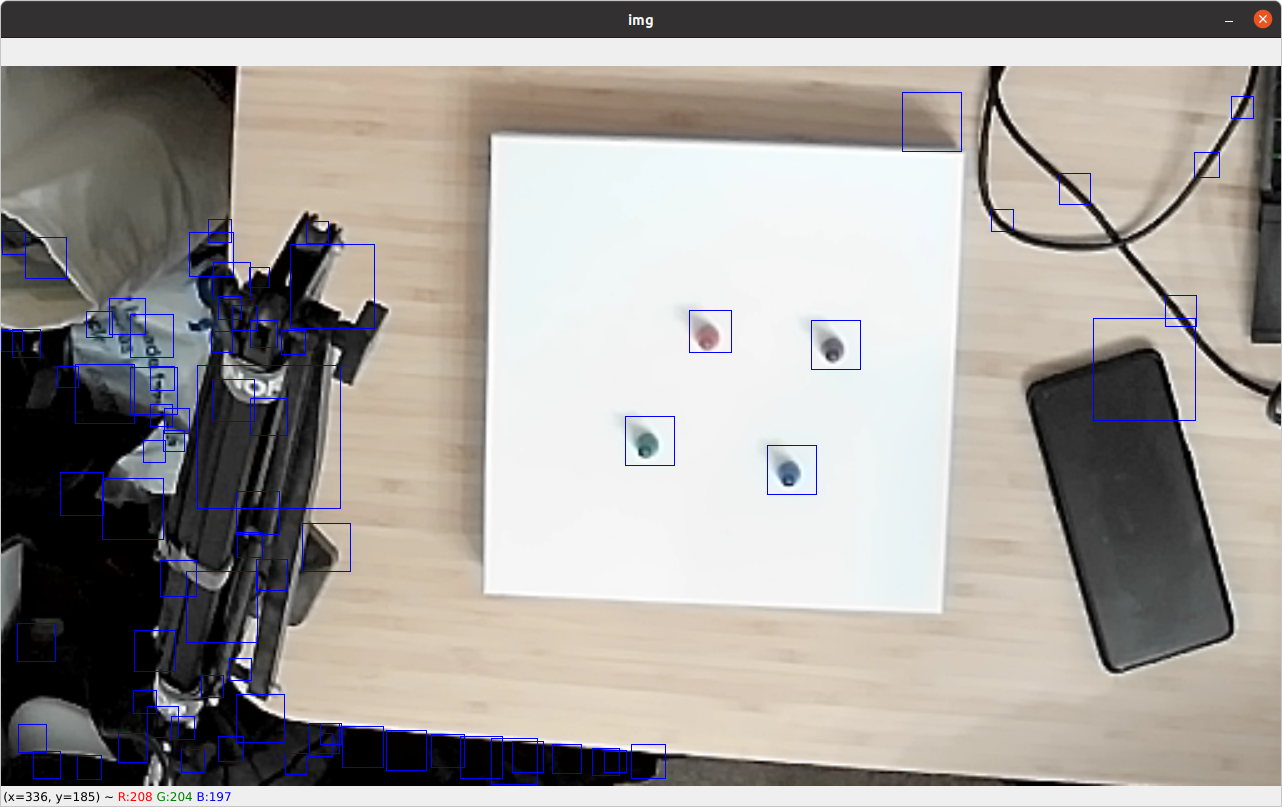
\includegraphics[width=\textwidth]{images/figures/app2a}
        \caption{Model 1}
        \label{fig:tokens1}
    \end{subfigure}
    \begin{subfigure}{1\textwidth}
        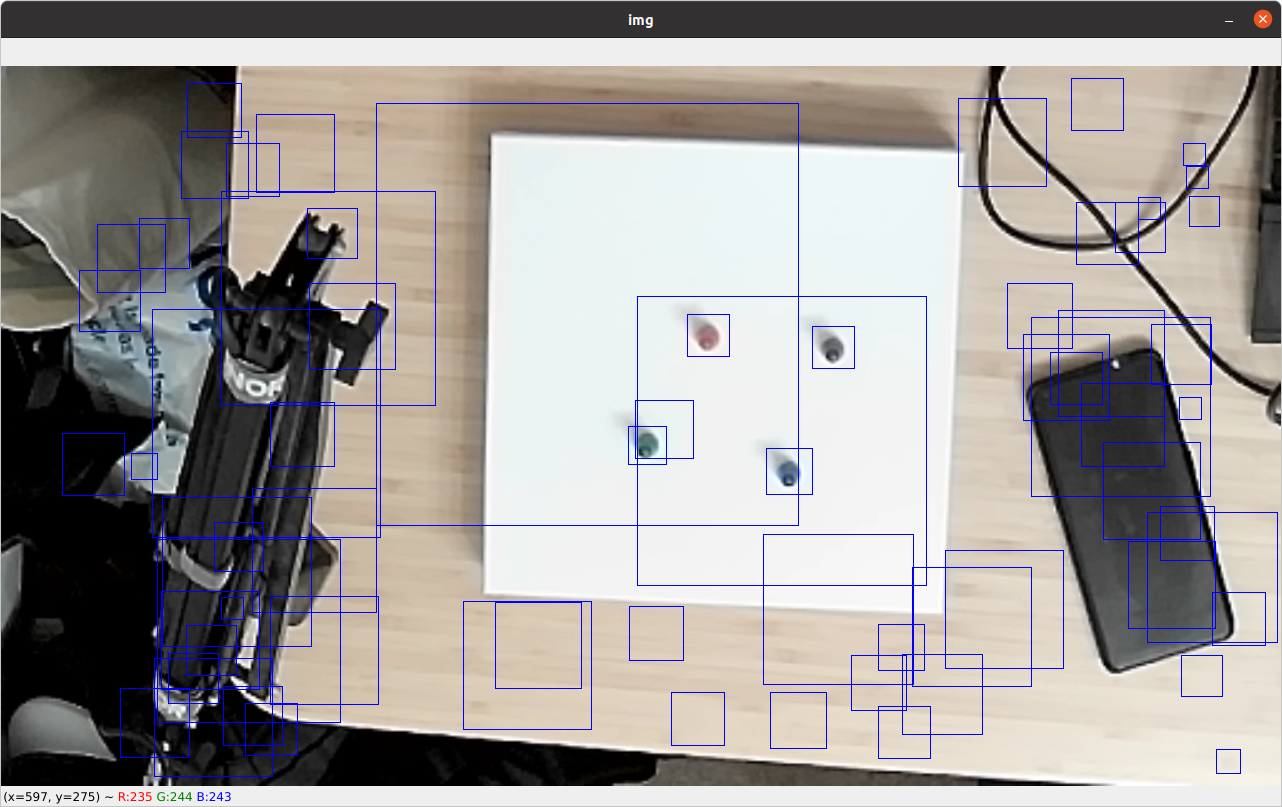
\includegraphics[width=\textwidth]{images/figures/app2b}
        \caption{Model 2}
        \label{fig:tokens2}
    \end{subfigure}
    \caption{Tokens Model 1 and 2 Test Results}
    \label{fig:main}
\end{figure}
\begin{figure}[H]
    \ContinuedFloat
    \begin{subfigure}{1\textwidth}
        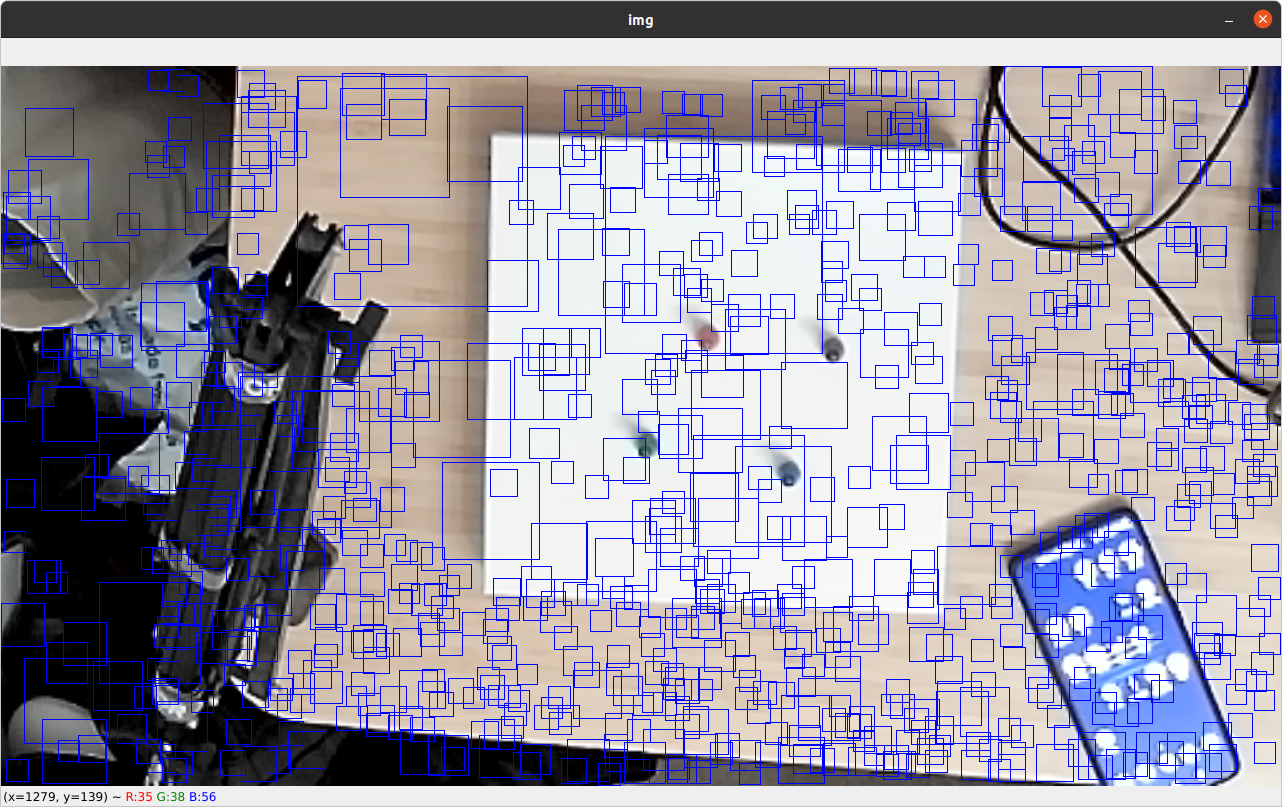
\includegraphics[width=\textwidth]{images/figures/app2c}
        \caption{Model 3}
        \label{fig:tokens3}
    \end{subfigure}
    \begin{subfigure}{1\textwidth}
        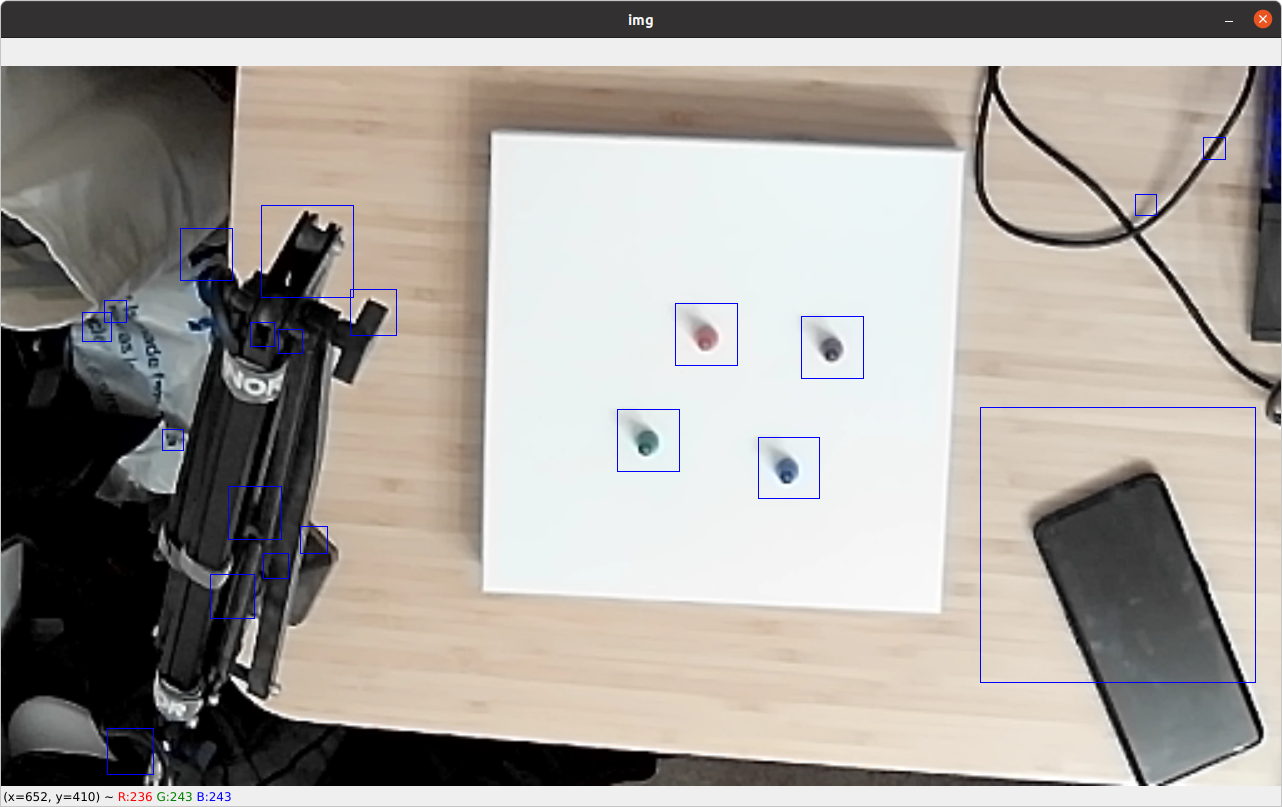
\includegraphics[width=\textwidth]{images/figures/app2d}
        \caption{Final Model}
        \label{fig:tokens4}
    \end{subfigure}
    
    \caption{Tokens Model 3 and Final Test Results}
    \label{fig:main}
\end{figure}


\addcontentsline{toc}{section}{References}
\printbibliography

%TC:endignore

\end{document}
